\documentclass[11pt]{article}
\usepackage[utf8]{inputenc}
\usepackage[T1]{fontenc}
\usepackage{lmodern}
\usepackage{geometry}
\geometry{margin=1in}
\usepackage{amsmath,amssymb}
\usepackage{booktabs}
\usepackage{tabularx}
\usepackage{graphicx}
\usepackage{microtype}
\usepackage[numbers]{natbib}
\usepackage{hyperref}
\hypersetup{hidelinks}

\newcommand{\eco}{\Delta_{\mathrm{eco}}}
\newcommand{\eli}{\Delta_{\mathrm{eli}}}
\newcommand{\soc}{\Delta_{\mathrm{soc}}}
\newcommand{\tot}{\Delta_{\mathrm{tot}}}
% Numbers are generated from the data by make_figures.py (tables/numbers.tex).
% Generated by make_figures.py; do not edit.
\expandafter\def\csname n@ad-qwen1930-A1930-favorA\endcsname{0.21}
\expandafter\def\csname n@ad-qwen1930-A1930-moralfict\endcsname{0.07}
\expandafter\def\csname n@ad-qwen1930-A1930-notreal\endcsname{0.42}
\expandafter\def\csname n@ad-qwen1930-A1930-practfict\endcsname{0.13}
\expandafter\def\csname n@ad-qwen1930-A1930-practreal\endcsname{0.40}
\expandafter\def\csname n@ad-qwen1930-A1930-real\endcsname{0.40}
\expandafter\def\csname n@ad-qwen1930-Dfull-favorA\endcsname{0.57}
\expandafter\def\csname n@ad-qwen1930-Dfull-moralfict\endcsname{0.34}
\expandafter\def\csname n@ad-qwen1930-Dfull-notreal\endcsname{0.74}
\expandafter\def\csname n@ad-qwen1930-Dfull-practfict\endcsname{0.32}
\expandafter\def\csname n@ad-qwen1930-Dfull-practreal\endcsname{0.54}
\expandafter\def\csname n@ad-qwen1930-Dfull-real\endcsname{0.52}
\expandafter\def\csname n@ad-qwen1930-Dpeers-favorA\endcsname{0.31}
\expandafter\def\csname n@ad-qwen1930-Dpeers-moralfict\endcsname{0.40}
\expandafter\def\csname n@ad-qwen1930-Dpeers-notreal\endcsname{0.76}
\expandafter\def\csname n@ad-qwen1930-Dpeers-practfict\endcsname{0.33}
\expandafter\def\csname n@ad-qwen1930-Dpeers-practreal\endcsname{0.37}
\expandafter\def\csname n@ad-qwen1930-Dpeers-real\endcsname{0.49}
\expandafter\def\csname n@ad-qwen1930-eco-favorA\endcsname{-0.04}
\expandafter\def\csname n@ad-qwen1930-eco-favorA-ci\endcsname{[-0.27,+0.17]}
\expandafter\def\csname n@ad-qwen1930-eco-favorA-n\endcsname{8}
\expandafter\def\csname n@ad-qwen1930-eco-moralfict\endcsname{+0.18}
\expandafter\def\csname n@ad-qwen1930-eco-moralfict-ci\endcsname{[+0.03,+0.37]}
\expandafter\def\csname n@ad-qwen1930-eco-moralfict-n\endcsname{10}
\expandafter\def\csname n@ad-qwen1930-eco-notreal\endcsname{+0.12}
\expandafter\def\csname n@ad-qwen1930-eco-notreal-ci\endcsname{[-0.15,+0.38]}
\expandafter\def\csname n@ad-qwen1930-eco-notreal-n\endcsname{8}
\expandafter\def\csname n@ad-qwen1930-eco-practfict\endcsname{+0.03}
\expandafter\def\csname n@ad-qwen1930-eco-practfict-ci\endcsname{[-0.13,+0.20]}
\expandafter\def\csname n@ad-qwen1930-eco-practfict-n\endcsname{10}
\expandafter\def\csname n@ad-qwen1930-eco-practreal\endcsname{+0.03}
\expandafter\def\csname n@ad-qwen1930-eco-practreal-ci\endcsname{[-0.18,+0.27]}
\expandafter\def\csname n@ad-qwen1930-eco-practreal-n\endcsname{10}
\expandafter\def\csname n@ad-qwen1930-eco-real\endcsname{+0.03}
\expandafter\def\csname n@ad-qwen1930-eco-real-ci\endcsname{[-0.08,+0.14]}
\expandafter\def\csname n@ad-qwen1930-eco-real-n\endcsname{35}
\expandafter\def\csname n@ad-qwen1930-peers-favorA\endcsname{+0.03}
\expandafter\def\csname n@ad-qwen1930-peers-favorA-ci\endcsname{[-0.16,+0.22]}
\expandafter\def\csname n@ad-qwen1930-peers-favorA-n\endcsname{8}
\expandafter\def\csname n@ad-qwen1930-peers-moralfict\endcsname{+0.16}
\expandafter\def\csname n@ad-qwen1930-peers-moralfict-ci\endcsname{[+0.01,+0.32]}
\expandafter\def\csname n@ad-qwen1930-peers-moralfict-n\endcsname{9}
\expandafter\def\csname n@ad-qwen1930-peers-notreal\endcsname{+0.19}
\expandafter\def\csname n@ad-qwen1930-peers-notreal-ci\endcsname{[+0.07,+0.30]}
\expandafter\def\csname n@ad-qwen1930-peers-notreal-n\endcsname{8}
\expandafter\def\csname n@ad-qwen1930-peers-practfict\endcsname{+0.07}
\expandafter\def\csname n@ad-qwen1930-peers-practfict-ci\endcsname{[-0.02,+0.17]}
\expandafter\def\csname n@ad-qwen1930-peers-practfict-n\endcsname{10}
\expandafter\def\csname n@ad-qwen1930-peers-practreal\endcsname{-0.05}
\expandafter\def\csname n@ad-qwen1930-peers-practreal-ci\endcsname{[-0.29,+0.22]}
\expandafter\def\csname n@ad-qwen1930-peers-practreal-n\endcsname{9}
\expandafter\def\csname n@ad-qwen1930-peers-real\endcsname{+0.03}
\expandafter\def\csname n@ad-qwen1930-peers-real-ci\endcsname{[-0.08,+0.14]}
\expandafter\def\csname n@ad-qwen1930-peers-real-n\endcsname{33}
\expandafter\def\csname n@ad-qwen1930-tot-favorA\endcsname{+0.33}
\expandafter\def\csname n@ad-qwen1930-tot-favorA-ci\endcsname{[+0.21,+0.48]}
\expandafter\def\csname n@ad-qwen1930-tot-favorA-n\endcsname{7}
\expandafter\def\csname n@ad-qwen1930-tot-moralfict\endcsname{+0.28}
\expandafter\def\csname n@ad-qwen1930-tot-moralfict-ci\endcsname{[+0.08,+0.50]}
\expandafter\def\csname n@ad-qwen1930-tot-moralfict-n\endcsname{10}
\expandafter\def\csname n@ad-qwen1930-tot-notreal\endcsname{+0.32}
\expandafter\def\csname n@ad-qwen1930-tot-notreal-ci\endcsname{[+0.12,+0.50]}
\expandafter\def\csname n@ad-qwen1930-tot-notreal-n\endcsname{8}
\expandafter\def\csname n@ad-qwen1930-tot-practfict\endcsname{+0.21}
\expandafter\def\csname n@ad-qwen1930-tot-practfict-ci\endcsname{[-0.04,+0.46]}
\expandafter\def\csname n@ad-qwen1930-tot-practfict-n\endcsname{9}
\expandafter\def\csname n@ad-qwen1930-tot-practreal\endcsname{+0.20}
\expandafter\def\csname n@ad-qwen1930-tot-practreal-ci\endcsname{[+0.02,+0.42]}
\expandafter\def\csname n@ad-qwen1930-tot-practreal-n\endcsname{10}
\expandafter\def\csname n@ad-qwen1930-tot-real\endcsname{+0.14}
\expandafter\def\csname n@ad-qwen1930-tot-real-ci\endcsname{[+0.01,+0.27]}
\expandafter\def\csname n@ad-qwen1930-tot-real-n\endcsname{34}
\expandafter\def\csname n@ad-qwen1930-totpeers-favorA\endcsname{+0.12}
\expandafter\def\csname n@ad-qwen1930-totpeers-favorA-ci\endcsname{[+0.04,+0.23]}
\expandafter\def\csname n@ad-qwen1930-totpeers-favorA-n\endcsname{8}
\expandafter\def\csname n@ad-qwen1930-totpeers-moralfict\endcsname{+0.33}
\expandafter\def\csname n@ad-qwen1930-totpeers-moralfict-ci\endcsname{[+0.13,+0.53]}
\expandafter\def\csname n@ad-qwen1930-totpeers-moralfict-n\endcsname{10}
\expandafter\def\csname n@ad-qwen1930-totpeers-notreal\endcsname{+0.34}
\expandafter\def\csname n@ad-qwen1930-totpeers-notreal-ci\endcsname{[+0.17,+0.53]}
\expandafter\def\csname n@ad-qwen1930-totpeers-notreal-n\endcsname{8}
\expandafter\def\csname n@ad-qwen1930-totpeers-practfict\endcsname{+0.23}
\expandafter\def\csname n@ad-qwen1930-totpeers-practfict-ci\endcsname{[+0.02,+0.43]}
\expandafter\def\csname n@ad-qwen1930-totpeers-practfict-n\endcsname{10}
\expandafter\def\csname n@ad-qwen1930-totpeers-practreal\endcsname{-0.04}
\expandafter\def\csname n@ad-qwen1930-totpeers-practreal-ci\endcsname{[-0.22,+0.15]}
\expandafter\def\csname n@ad-qwen1930-totpeers-practreal-n\endcsname{9}
\expandafter\def\csname n@ad-qwen1930-totpeers-real\endcsname{+0.07}
\expandafter\def\csname n@ad-qwen1930-totpeers-real-ci\endcsname{[-0.04,+0.19]}
\expandafter\def\csname n@ad-qwen1930-totpeers-real-n\endcsname{34}
\expandafter\def\csname n@ad-talkie-A1930-favorA\endcsname{0.31}
\expandafter\def\csname n@ad-talkie-A1930-moralfict\endcsname{0.37}
\expandafter\def\csname n@ad-talkie-A1930-notreal\endcsname{0.42}
\expandafter\def\csname n@ad-talkie-A1930-practfict\endcsname{0.07}
\expandafter\def\csname n@ad-talkie-A1930-practreal\endcsname{0.40}
\expandafter\def\csname n@ad-talkie-A1930-real\endcsname{0.40}
\expandafter\def\csname n@ad-talkie-Dfull-favorA\endcsname{0.77}
\expandafter\def\csname n@ad-talkie-Dfull-moralfict\endcsname{0.73}
\expandafter\def\csname n@ad-talkie-Dfull-notreal\endcsname{0.96}
\expandafter\def\csname n@ad-talkie-Dfull-practfict\endcsname{0.35}
\expandafter\def\csname n@ad-talkie-Dfull-practreal\endcsname{0.77}
\expandafter\def\csname n@ad-talkie-Dfull-real\endcsname{0.86}
\expandafter\def\csname n@ad-talkie-Dpeers-favorA\endcsname{0.79}
\expandafter\def\csname n@ad-talkie-Dpeers-moralfict\endcsname{0.87}
\expandafter\def\csname n@ad-talkie-Dpeers-notreal\endcsname{1.00}
\expandafter\def\csname n@ad-talkie-Dpeers-practfict\endcsname{0.15}
\expandafter\def\csname n@ad-talkie-Dpeers-practreal\endcsname{0.93}
\expandafter\def\csname n@ad-talkie-Dpeers-real\endcsname{0.88}
\expandafter\def\csname n@ad-talkie-eco-favorA\endcsname{+0.06}
\expandafter\def\csname n@ad-talkie-eco-favorA-ci\endcsname{[-0.08,+0.19]}
\expandafter\def\csname n@ad-talkie-eco-favorA-n\endcsname{8}
\expandafter\def\csname n@ad-talkie-eco-moralfict\endcsname{-0.07}
\expandafter\def\csname n@ad-talkie-eco-moralfict-ci\endcsname{[-0.30,+0.13]}
\expandafter\def\csname n@ad-talkie-eco-moralfict-n\endcsname{10}
\expandafter\def\csname n@ad-talkie-eco-notreal\endcsname{+0.08}
\expandafter\def\csname n@ad-talkie-eco-notreal-ci\endcsname{[0.00,+0.25]}
\expandafter\def\csname n@ad-talkie-eco-notreal-n\endcsname{8}
\expandafter\def\csname n@ad-talkie-eco-practfict\endcsname{-0.07}
\expandafter\def\csname n@ad-talkie-eco-practfict-ci\endcsname{[-0.20,0.00]}
\expandafter\def\csname n@ad-talkie-eco-practfict-n\endcsname{10}
\expandafter\def\csname n@ad-talkie-eco-practreal\endcsname{-0.13}
\expandafter\def\csname n@ad-talkie-eco-practreal-ci\endcsname{[-0.43,+0.13]}
\expandafter\def\csname n@ad-talkie-eco-practreal-n\endcsname{10}
\expandafter\def\csname n@ad-talkie-eco-real\endcsname{+0.07}
\expandafter\def\csname n@ad-talkie-eco-real-ci\endcsname{[-0.06,+0.21]}
\expandafter\def\csname n@ad-talkie-eco-real-n\endcsname{35}
\expandafter\def\csname n@ad-talkie-peers-favorA\endcsname{+0.31}
\expandafter\def\csname n@ad-talkie-peers-favorA-ci\endcsname{[+0.10,+0.56]}
\expandafter\def\csname n@ad-talkie-peers-favorA-n\endcsname{8}
\expandafter\def\csname n@ad-talkie-peers-moralfict\endcsname{+0.23}
\expandafter\def\csname n@ad-talkie-peers-moralfict-ci\endcsname{[+0.08,+0.40]}
\expandafter\def\csname n@ad-talkie-peers-moralfict-n\endcsname{10}
\expandafter\def\csname n@ad-talkie-peers-notreal\endcsname{+0.33}
\expandafter\def\csname n@ad-talkie-peers-notreal-ci\endcsname{[+0.08,+0.67]}
\expandafter\def\csname n@ad-talkie-peers-notreal-n\endcsname{8}
\expandafter\def\csname n@ad-talkie-peers-practfict\endcsname{+0.02}
\expandafter\def\csname n@ad-talkie-peers-practfict-ci\endcsname{[-0.05,+0.10]}
\expandafter\def\csname n@ad-talkie-peers-practfict-n\endcsname{10}
\expandafter\def\csname n@ad-talkie-peers-practreal\endcsname{+0.67}
\expandafter\def\csname n@ad-talkie-peers-practreal-ci\endcsname{[+0.40,+0.90]}
\expandafter\def\csname n@ad-talkie-peers-practreal-n\endcsname{10}
\expandafter\def\csname n@ad-talkie-peers-real\endcsname{+0.30}
\expandafter\def\csname n@ad-talkie-peers-real-ci\endcsname{[+0.16,+0.45]}
\expandafter\def\csname n@ad-talkie-peers-real-n\endcsname{35}
\expandafter\def\csname n@ad-talkie-tot-favorA\endcsname{+0.46}
\expandafter\def\csname n@ad-talkie-tot-favorA-ci\endcsname{[+0.23,+0.67]}
\expandafter\def\csname n@ad-talkie-tot-favorA-n\endcsname{8}
\expandafter\def\csname n@ad-talkie-tot-moralfict\endcsname{+0.37}
\expandafter\def\csname n@ad-talkie-tot-moralfict-ci\endcsname{[+0.13,+0.60]}
\expandafter\def\csname n@ad-talkie-tot-moralfict-n\endcsname{10}
\expandafter\def\csname n@ad-talkie-tot-notreal\endcsname{+0.54}
\expandafter\def\csname n@ad-talkie-tot-notreal-ci\endcsname{[+0.29,+0.79]}
\expandafter\def\csname n@ad-talkie-tot-notreal-n\endcsname{8}
\expandafter\def\csname n@ad-talkie-tot-practfict\endcsname{+0.28}
\expandafter\def\csname n@ad-talkie-tot-practfict-ci\endcsname{[-0.02,+0.60]}
\expandafter\def\csname n@ad-talkie-tot-practfict-n\endcsname{10}
\expandafter\def\csname n@ad-talkie-tot-practreal\endcsname{+0.37}
\expandafter\def\csname n@ad-talkie-tot-practreal-ci\endcsname{[+0.17,+0.57]}
\expandafter\def\csname n@ad-talkie-tot-practreal-n\endcsname{10}
\expandafter\def\csname n@ad-talkie-tot-real\endcsname{+0.47}
\expandafter\def\csname n@ad-talkie-tot-real-ci\endcsname{[+0.34,+0.60]}
\expandafter\def\csname n@ad-talkie-tot-real-n\endcsname{35}
\expandafter\def\csname n@ad-talkie-totpeers-favorA\endcsname{+0.48}
\expandafter\def\csname n@ad-talkie-totpeers-favorA-ci\endcsname{[+0.23,+0.71]}
\expandafter\def\csname n@ad-talkie-totpeers-favorA-n\endcsname{8}
\expandafter\def\csname n@ad-talkie-totpeers-moralfict\endcsname{+0.47}
\expandafter\def\csname n@ad-talkie-totpeers-moralfict-ci\endcsname{[+0.20,+0.73]}
\expandafter\def\csname n@ad-talkie-totpeers-moralfict-n\endcsname{10}
\expandafter\def\csname n@ad-talkie-totpeers-notreal\endcsname{+0.58}
\expandafter\def\csname n@ad-talkie-totpeers-notreal-ci\endcsname{[+0.29,+0.83]}
\expandafter\def\csname n@ad-talkie-totpeers-notreal-n\endcsname{8}
\expandafter\def\csname n@ad-talkie-totpeers-practfict\endcsname{+0.08}
\expandafter\def\csname n@ad-talkie-totpeers-practfict-ci\endcsname{[-0.15,+0.33]}
\expandafter\def\csname n@ad-talkie-totpeers-practfict-n\endcsname{10}
\expandafter\def\csname n@ad-talkie-totpeers-practreal\endcsname{+0.53}
\expandafter\def\csname n@ad-talkie-totpeers-practreal-ci\endcsname{[+0.30,+0.77]}
\expandafter\def\csname n@ad-talkie-totpeers-practreal-n\endcsname{10}
\expandafter\def\csname n@ad-talkie-totpeers-real\endcsname{+0.49}
\expandafter\def\csname n@ad-talkie-totpeers-real-ci\endcsname{[+0.36,+0.62]}
\expandafter\def\csname n@ad-talkie-totpeers-real-n\endcsname{35}
\expandafter\def\csname n@b-diff-direction\endcsname{+0.31}
\expandafter\def\csname n@b-diff-direction-ci\endcsname{[+0.22,+0.41]}
\expandafter\def\csname n@b-diff-direction-n\endcsname{69}
\expandafter\def\csname n@b-diff-eli\endcsname{+0.14}
\expandafter\def\csname n@b-diff-eli-ci\endcsname{[+0.04,+0.24]}
\expandafter\def\csname n@b-diff-eli-n\endcsname{72}
\expandafter\def\csname n@b-diff-inst\endcsname{0.00}
\expandafter\def\csname n@b-diff-inst-ci\endcsname{[-0.12,+0.13]}
\expandafter\def\csname n@b-diff-inst-n\endcsname{65}
\expandafter\def\csname n@b-diff-media\endcsname{-0.03}
\expandafter\def\csname n@b-diff-media-ci\endcsname{[-0.12,+0.05]}
\expandafter\def\csname n@b-diff-media-n\endcsname{63}
\expandafter\def\csname n@b-diff-moralclaim\endcsname{+0.23}
\expandafter\def\csname n@b-diff-moralclaim-ci\endcsname{[+0.13,+0.33]}
\expandafter\def\csname n@b-diff-moralclaim-n\endcsname{67}
\expandafter\def\csname n@b-diff-opacity\endcsname{-0.01}
\expandafter\def\csname n@b-diff-opacity-ci\endcsname{[-0.11,+0.08]}
\expandafter\def\csname n@b-diff-opacity-n\endcsname{69}
\expandafter\def\csname n@b-diff-peers\endcsname{+0.20}
\expandafter\def\csname n@b-diff-peers-ci\endcsname{[+0.08,+0.31]}
\expandafter\def\csname n@b-diff-peers-n\endcsname{68}
\expandafter\def\csname n@b-diff-pullback\endcsname{+0.15}
\expandafter\def\csname n@b-diff-pullback-ci\endcsname{[+0.06,+0.24]}
\expandafter\def\csname n@b-diff-pullback-n\endcsname{71}
\expandafter\def\csname n@b-qwen1930-direction\endcsname{+0.02}
\expandafter\def\csname n@b-qwen1930-direction-ci\endcsname{[-0.05,+0.08]}
\expandafter\def\csname n@b-qwen1930-direction-n\endcsname{69}
\expandafter\def\csname n@b-qwen1930-eli\endcsname{+0.01}
\expandafter\def\csname n@b-qwen1930-eli-ci\endcsname{[-0.05,+0.06]}
\expandafter\def\csname n@b-qwen1930-eli-n\endcsname{72}
\expandafter\def\csname n@b-qwen1930-inst\endcsname{+0.02}
\expandafter\def\csname n@b-qwen1930-inst-ci\endcsname{[-0.07,+0.09]}
\expandafter\def\csname n@b-qwen1930-inst-n\endcsname{65}
\expandafter\def\csname n@b-qwen1930-media\endcsname{0.00}
\expandafter\def\csname n@b-qwen1930-media-ci\endcsname{[-0.06,+0.06]}
\expandafter\def\csname n@b-qwen1930-media-n\endcsname{65}
\expandafter\def\csname n@b-qwen1930-moralclaim\endcsname{+0.02}
\expandafter\def\csname n@b-qwen1930-moralclaim-ci\endcsname{[-0.04,+0.08]}
\expandafter\def\csname n@b-qwen1930-moralclaim-n\endcsname{67}
\expandafter\def\csname n@b-qwen1930-opacity\endcsname{-0.10}
\expandafter\def\csname n@b-qwen1930-opacity-ci\endcsname{[-0.16,-0.04]}
\expandafter\def\csname n@b-qwen1930-opacity-n\endcsname{69}
\expandafter\def\csname n@b-qwen1930-peers\endcsname{+0.06}
\expandafter\def\csname n@b-qwen1930-peers-ci\endcsname{[-0.01,+0.12]}
\expandafter\def\csname n@b-qwen1930-peers-n\endcsname{69}
\expandafter\def\csname n@b-qwen1930-pullback\endcsname{+0.02}
\expandafter\def\csname n@b-qwen1930-pullback-ci\endcsname{[-0.03,+0.08]}
\expandafter\def\csname n@b-qwen1930-pullback-n\endcsname{71}
\expandafter\def\csname n@b-talkie-direction\endcsname{+0.32}
\expandafter\def\csname n@b-talkie-direction-ci\endcsname{[+0.25,+0.40]}
\expandafter\def\csname n@b-talkie-direction-n\endcsname{72}
\expandafter\def\csname n@b-talkie-eli\endcsname{+0.15}
\expandafter\def\csname n@b-talkie-eli-ci\endcsname{[+0.07,+0.22]}
\expandafter\def\csname n@b-talkie-eli-n\endcsname{72}
\expandafter\def\csname n@b-talkie-inst\endcsname{+0.01}
\expandafter\def\csname n@b-talkie-inst-ci\endcsname{[-0.06,+0.09]}
\expandafter\def\csname n@b-talkie-inst-n\endcsname{72}
\expandafter\def\csname n@b-talkie-media\endcsname{-0.04}
\expandafter\def\csname n@b-talkie-media-ci\endcsname{[-0.10,+0.02]}
\expandafter\def\csname n@b-talkie-media-n\endcsname{70}
\expandafter\def\csname n@b-talkie-moralclaim\endcsname{+0.25}
\expandafter\def\csname n@b-talkie-moralclaim-ci\endcsname{[+0.17,+0.33]}
\expandafter\def\csname n@b-talkie-moralclaim-n\endcsname{72}
\expandafter\def\csname n@b-talkie-opacity\endcsname{-0.11}
\expandafter\def\csname n@b-talkie-opacity-ci\endcsname{[-0.19,-0.04]}
\expandafter\def\csname n@b-talkie-opacity-n\endcsname{72}
\expandafter\def\csname n@b-talkie-peers\endcsname{+0.27}
\expandafter\def\csname n@b-talkie-peers-ci\endcsname{[+0.19,+0.37]}
\expandafter\def\csname n@b-talkie-peers-n\endcsname{71}
\expandafter\def\csname n@b-talkie-pullback\endcsname{+0.17}
\expandafter\def\csname n@b-talkie-pullback-ci\endcsname{[+0.10,+0.25]}
\expandafter\def\csname n@b-talkie-pullback-n\endcsname{72}
\expandafter\def\csname n@cap-qwen1930-hit\endcsname{1777}
\expandafter\def\csname n@cap-qwen1930-n\endcsname{1944}
\expandafter\def\csname n@cap-talkie-hit\endcsname{21}
\expandafter\def\csname n@cap-talkie-n\endcsname{1944}
\expandafter\def\csname n@cue-agree\endcsname{94}
\expandafter\def\csname n@cue-agree4\endcsname{76}
\expandafter\def\csname n@cue-diff\endcsname{-0.13}
\expandafter\def\csname n@cue-diff-ci\endcsname{[-0.24,-0.01]}
\expandafter\def\csname n@cue-diff-n\endcsname{68}
\expandafter\def\csname n@cue-n\endcsname{1296}
\expandafter\def\csname n@e-source\endcsname{e_all_r3}
\expandafter\def\csname n@n-balanced\endcsname{40}
\expandafter\def\csname n@n-domains\endcsname{72}
\expandafter\def\csname n@n-favorA\endcsname{8}
\expandafter\def\csname n@n-favorB\endcsname{16}
\expandafter\def\csname n@n-fictional\endcsname{20}
\expandafter\def\csname n@n-hanson\endcsname{8}
\expandafter\def\csname n@n-interviews\endcsname{3888}
\expandafter\def\csname n@n-notreal\endcsname{8}
\expandafter\def\csname n@n-partial\endcsname{9}
\expandafter\def\csname n@n-planned\endcsname{3888}
\expandafter\def\csname n@n-real\endcsname{35}
\expandafter\def\csname n@qwen1930-any-A1930\endcsname{0.87}
\expandafter\def\csname n@qwen1930-any-Btransplant\endcsname{0.82}
\expandafter\def\csname n@qwen1930-any-Celites\endcsname{0.69}
\expandafter\def\csname n@qwen1930-any-Dfull\endcsname{0.66}
\expandafter\def\csname n@qwen1930-any-Dpeers\endcsname{0.67}
\expandafter\def\csname n@qwen1930-cue-absent\endcsname{1--7}
\expandafter\def\csname n@qwen1930-cue-absent-against\endcsname{3--7}
\expandafter\def\csname n@qwen1930-cue-judge\endcsname{2}
\expandafter\def\csname n@qwen1930-cue-n\endcsname{211}
\expandafter\def\csname n@qwen1930-cue-reason\endcsname{49}
\expandafter\def\csname n@qwen1930-cue-rejected\endcsname{20--45}
\expandafter\def\csname n@qwen1930-direction-balanced\endcsname{+0.02}
\expandafter\def\csname n@qwen1930-direction-balanced-ci\endcsname{[-0.07,+0.11]}
\expandafter\def\csname n@qwen1930-direction-balanced-n\endcsname{39}
\expandafter\def\csname n@qwen1930-direction-favorA\endcsname{+0.01}
\expandafter\def\csname n@qwen1930-direction-favorA-ci\endcsname{[-0.07,+0.11]}
\expandafter\def\csname n@qwen1930-direction-favorA-n\endcsname{7}
\expandafter\def\csname n@qwen1930-direction-favorB\endcsname{+0.04}
\expandafter\def\csname n@qwen1930-direction-favorB-ci\endcsname{[-0.17,+0.21]}
\expandafter\def\csname n@qwen1930-direction-favorB-n\endcsname{15}
\expandafter\def\csname n@qwen1930-direction-hanson\endcsname{-0.02}
\expandafter\def\csname n@qwen1930-direction-hanson-ci\endcsname{[-0.21,+0.15]}
\expandafter\def\csname n@qwen1930-direction-hanson-n\endcsname{8}
\expandafter\def\csname n@qwen1930-eco-all\endcsname{+0.08}
\expandafter\def\csname n@qwen1930-eco-all-ci\endcsname{[+0.01,+0.16]}
\expandafter\def\csname n@qwen1930-eco-all-n\endcsname{72}
\expandafter\def\csname n@qwen1930-eco-balanced\endcsname{+0.05}
\expandafter\def\csname n@qwen1930-eco-balanced-ci\endcsname{[-0.04,+0.15]}
\expandafter\def\csname n@qwen1930-eco-balanced-n\endcsname{40}
\expandafter\def\csname n@qwen1930-eco-favorA\endcsname{-0.04}
\expandafter\def\csname n@qwen1930-eco-favorA-ci\endcsname{[-0.25,+0.17]}
\expandafter\def\csname n@qwen1930-eco-favorA-n\endcsname{8}
\expandafter\def\csname n@qwen1930-eco-favorB\endcsname{+0.16}
\expandafter\def\csname n@qwen1930-eco-favorB-ci\endcsname{[+0.02,+0.30]}
\expandafter\def\csname n@qwen1930-eco-favorB-n\endcsname{16}
\expandafter\def\csname n@qwen1930-eco-hanson\endcsname{+0.20}
\expandafter\def\csname n@qwen1930-eco-hanson-ci\endcsname{[-0.03,+0.48]}
\expandafter\def\csname n@qwen1930-eco-hanson-n\endcsname{8}
\expandafter\def\csname n@qwen1930-eco-real\endcsname{+0.03}
\expandafter\def\csname n@qwen1930-eco-real-ci\endcsname{[-0.08,+0.14]}
\expandafter\def\csname n@qwen1930-eco-real-n\endcsname{35}
\expandafter\def\csname n@qwen1930-eli-all\endcsname{+0.01}
\expandafter\def\csname n@qwen1930-eli-all-ci\endcsname{[-0.05,+0.06]}
\expandafter\def\csname n@qwen1930-eli-all-n\endcsname{72}
\expandafter\def\csname n@qwen1930-eli-balanced\endcsname{-0.01}
\expandafter\def\csname n@qwen1930-eli-balanced-ci\endcsname{[-0.08,+0.07]}
\expandafter\def\csname n@qwen1930-eli-balanced-n\endcsname{40}
\expandafter\def\csname n@qwen1930-eli-favorA\endcsname{+0.07}
\expandafter\def\csname n@qwen1930-eli-favorA-ci\endcsname{[-0.04,+0.22]}
\expandafter\def\csname n@qwen1930-eli-favorA-n\endcsname{8}
\expandafter\def\csname n@qwen1930-eli-favorB\endcsname{+0.02}
\expandafter\def\csname n@qwen1930-eli-favorB-ci\endcsname{[-0.09,+0.14]}
\expandafter\def\csname n@qwen1930-eli-favorB-n\endcsname{16}
\expandafter\def\csname n@qwen1930-eli-hanson\endcsname{-0.01}
\expandafter\def\csname n@qwen1930-eli-hanson-ci\endcsname{[-0.32,+0.19]}
\expandafter\def\csname n@qwen1930-eli-hanson-n\endcsname{8}
\expandafter\def\csname n@qwen1930-eli-real\endcsname{-0.01}
\expandafter\def\csname n@qwen1930-eli-real-ci\endcsname{[-0.11,+0.08]}
\expandafter\def\csname n@qwen1930-eli-real-n\endcsname{35}
\expandafter\def\csname n@qwen1930-level-all-A1930\endcsname{0.30}
\expandafter\def\csname n@qwen1930-level-all-Btransplant\endcsname{0.38}
\expandafter\def\csname n@qwen1930-level-all-Celites\endcsname{0.39}
\expandafter\def\csname n@qwen1930-level-all-Cexplained\endcsname{0.51}
\expandafter\def\csname n@qwen1930-level-all-Cmoral\endcsname{0.42}
\expandafter\def\csname n@qwen1930-level-all-Copposite\endcsname{0.36}
\expandafter\def\csname n@qwen1930-level-all-Dfull\endcsname{0.51}
\expandafter\def\csname n@qwen1930-level-all-Dmedia\endcsname{0.52}
\expandafter\def\csname n@qwen1930-level-all-Dpeers\endcsname{0.48}
\expandafter\def\csname n@qwen1930-level-balanced-A1930\endcsname{0.23}
\expandafter\def\csname n@qwen1930-level-balanced-Btransplant\endcsname{0.28}
\expandafter\def\csname n@qwen1930-level-balanced-Celites\endcsname{0.29}
\expandafter\def\csname n@qwen1930-level-balanced-Cexplained\endcsname{0.42}
\expandafter\def\csname n@qwen1930-level-balanced-Cmoral\endcsname{0.32}
\expandafter\def\csname n@qwen1930-level-balanced-Copposite\endcsname{0.26}
\expandafter\def\csname n@qwen1930-level-balanced-Dfull\endcsname{0.41}
\expandafter\def\csname n@qwen1930-level-balanced-Dmedia\endcsname{0.43}
\expandafter\def\csname n@qwen1930-level-balanced-Dpeers\endcsname{0.37}
\expandafter\def\csname n@qwen1930-level-favorA-A1930\endcsname{0.21}
\expandafter\def\csname n@qwen1930-level-favorA-Btransplant\endcsname{0.17}
\expandafter\def\csname n@qwen1930-level-favorA-Celites\endcsname{0.20}
\expandafter\def\csname n@qwen1930-level-favorA-Cexplained\endcsname{0.44}
\expandafter\def\csname n@qwen1930-level-favorA-Cmoral\endcsname{0.34}
\expandafter\def\csname n@qwen1930-level-favorA-Copposite\endcsname{0.27}
\expandafter\def\csname n@qwen1930-level-favorA-Dfull\endcsname{0.57}
\expandafter\def\csname n@qwen1930-level-favorA-Dmedia\endcsname{0.42}
\expandafter\def\csname n@qwen1930-level-favorA-Dpeers\endcsname{0.31}
\expandafter\def\csname n@qwen1930-level-favorB-A1930\endcsname{0.52}
\expandafter\def\csname n@qwen1930-level-favorB-Btransplant\endcsname{0.68}
\expandafter\def\csname n@qwen1930-level-favorB-Celites\endcsname{0.68}
\expandafter\def\csname n@qwen1930-level-favorB-Cexplained\endcsname{0.72}
\expandafter\def\csname n@qwen1930-level-favorB-Cmoral\endcsname{0.62}
\expandafter\def\csname n@qwen1930-level-favorB-Copposite\endcsname{0.56}
\expandafter\def\csname n@qwen1930-level-favorB-Dfull\endcsname{0.68}
\expandafter\def\csname n@qwen1930-level-favorB-Dmedia\endcsname{0.72}
\expandafter\def\csname n@qwen1930-level-favorB-Dpeers\endcsname{0.74}
\expandafter\def\csname n@qwen1930-level-hanson-A1930\endcsname{0.33}
\expandafter\def\csname n@qwen1930-level-hanson-Btransplant\endcsname{0.52}
\expandafter\def\csname n@qwen1930-level-hanson-Celites\endcsname{0.52}
\expandafter\def\csname n@qwen1930-level-hanson-Cexplained\endcsname{0.62}
\expandafter\def\csname n@qwen1930-level-hanson-Cmoral\endcsname{0.56}
\expandafter\def\csname n@qwen1930-level-hanson-Copposite\endcsname{0.54}
\expandafter\def\csname n@qwen1930-level-hanson-Dfull\endcsname{0.57}
\expandafter\def\csname n@qwen1930-level-hanson-Dmedia\endcsname{0.69}
\expandafter\def\csname n@qwen1930-level-hanson-Dpeers\endcsname{0.65}
\expandafter\def\csname n@qwen1930-mdir-A1930\endcsname{0.39}
\expandafter\def\csname n@qwen1930-mdir-Btransplant\endcsname{0.43}
\expandafter\def\csname n@qwen1930-mdir-Celites\endcsname{0.48}
\expandafter\def\csname n@qwen1930-mdir-Dfull\endcsname{0.51}
\expandafter\def\csname n@qwen1930-mdir-Dpeers\endcsname{0.51}
\expandafter\def\csname n@qwen1930-moralclaim-balanced\endcsname{+0.02}
\expandafter\def\csname n@qwen1930-moralclaim-balanced-ci\endcsname{[-0.06,+0.11]}
\expandafter\def\csname n@qwen1930-moralclaim-balanced-n\endcsname{37}
\expandafter\def\csname n@qwen1930-moralclaim-favorA\endcsname{+0.13}
\expandafter\def\csname n@qwen1930-moralclaim-favorA-ci\endcsname{[+0.02,+0.27]}
\expandafter\def\csname n@qwen1930-moralclaim-favorA-n\endcsname{7}
\expandafter\def\csname n@qwen1930-moralclaim-favorB\endcsname{-0.08}
\expandafter\def\csname n@qwen1930-moralclaim-favorB-ci\endcsname{[-0.19,+0.03]}
\expandafter\def\csname n@qwen1930-moralclaim-favorB-n\endcsname{15}
\expandafter\def\csname n@qwen1930-moralclaim-hanson\endcsname{+0.09}
\expandafter\def\csname n@qwen1930-moralclaim-hanson-ci\endcsname{[-0.09,+0.38]}
\expandafter\def\csname n@qwen1930-moralclaim-hanson-n\endcsname{8}
\expandafter\def\csname n@qwen1930-peers-balanced\endcsname{+0.05}
\expandafter\def\csname n@qwen1930-peers-balanced-ci\endcsname{[-0.03,+0.14]}
\expandafter\def\csname n@qwen1930-peers-balanced-n\endcsname{37}
\expandafter\def\csname n@qwen1930-peers-favorA\endcsname{+0.03}
\expandafter\def\csname n@qwen1930-peers-favorA-ci\endcsname{[-0.16,+0.22]}
\expandafter\def\csname n@qwen1930-peers-favorA-n\endcsname{8}
\expandafter\def\csname n@qwen1930-peers-favorB\endcsname{+0.05}
\expandafter\def\csname n@qwen1930-peers-favorB-ci\endcsname{[-0.06,+0.16]}
\expandafter\def\csname n@qwen1930-peers-favorB-n\endcsname{16}
\expandafter\def\csname n@qwen1930-peers-hanson\endcsname{+0.11}
\expandafter\def\csname n@qwen1930-peers-hanson-ci\endcsname{[-0.07,+0.39]}
\expandafter\def\csname n@qwen1930-peers-hanson-n\endcsname{8}
\expandafter\def\csname n@qwen1930-pullback-balanced\endcsname{+0.01}
\expandafter\def\csname n@qwen1930-pullback-balanced-ci\endcsname{[-0.06,+0.09]}
\expandafter\def\csname n@qwen1930-pullback-balanced-n\endcsname{39}
\expandafter\def\csname n@qwen1930-pullback-favorA\endcsname{-0.10}
\expandafter\def\csname n@qwen1930-pullback-favorA-ci\endcsname{[-0.25,+0.02]}
\expandafter\def\csname n@qwen1930-pullback-favorA-n\endcsname{8}
\expandafter\def\csname n@qwen1930-pullback-favorB\endcsname{+0.14}
\expandafter\def\csname n@qwen1930-pullback-favorB-ci\endcsname{[+0.03,+0.27]}
\expandafter\def\csname n@qwen1930-pullback-favorB-n\endcsname{16}
\expandafter\def\csname n@qwen1930-pullback-hanson\endcsname{-0.03}
\expandafter\def\csname n@qwen1930-pullback-hanson-ci\endcsname{[-0.21,+0.16]}
\expandafter\def\csname n@qwen1930-pullback-hanson-n\endcsname{8}
\expandafter\def\csname n@qwen1930-rho-all\endcsname{0.60}
\expandafter\def\csname n@qwen1930-rho-balanced\endcsname{0.72}
\expandafter\def\csname n@qwen1930-rho-favorA\endcsname{1.14}
\expandafter\def\csname n@qwen1930-rho-favorB\endcsname{0.03}
\expandafter\def\csname n@qwen1930-rho-hanson\endcsname{0.17}
\expandafter\def\csname n@qwen1930-rho-real\endcsname{0.81}
\expandafter\def\csname n@qwen1930-soc-all\endcsname{+0.13}
\expandafter\def\csname n@qwen1930-soc-all-ci\endcsname{[+0.06,+0.21]}
\expandafter\def\csname n@qwen1930-soc-all-n\endcsname{67}
\expandafter\def\csname n@qwen1930-soc-balanced\endcsname{+0.18}
\expandafter\def\csname n@qwen1930-soc-balanced-ci\endcsname{[+0.10,+0.27]}
\expandafter\def\csname n@qwen1930-soc-balanced-n\endcsname{36}
\expandafter\def\csname n@qwen1930-soc-favorA\endcsname{+0.31}
\expandafter\def\csname n@qwen1930-soc-favorA-ci\endcsname{[+0.10,+0.57]}
\expandafter\def\csname n@qwen1930-soc-favorA-n\endcsname{7}
\expandafter\def\csname n@qwen1930-soc-favorB\endcsname{-0.02}
\expandafter\def\csname n@qwen1930-soc-favorB-ci\endcsname{[-0.21,+0.15]}
\expandafter\def\csname n@qwen1930-soc-favorB-n\endcsname{16}
\expandafter\def\csname n@qwen1930-soc-hanson\endcsname{+0.09}
\expandafter\def\csname n@qwen1930-soc-hanson-ci\endcsname{[-0.12,+0.39]}
\expandafter\def\csname n@qwen1930-soc-hanson-n\endcsname{8}
\expandafter\def\csname n@qwen1930-soc-real\endcsname{+0.14}
\expandafter\def\csname n@qwen1930-soc-real-ci\endcsname{[+0.01,+0.27]}
\expandafter\def\csname n@qwen1930-soc-real-n\endcsname{32}
\expandafter\def\csname n@qwen1930-tot-all\endcsname{+0.21}
\expandafter\def\csname n@qwen1930-tot-all-ci\endcsname{[+0.13,+0.30]}
\expandafter\def\csname n@qwen1930-tot-all-n\endcsname{69}
\expandafter\def\csname n@qwen1930-tot-balanced\endcsname{+0.21}
\expandafter\def\csname n@qwen1930-tot-balanced-ci\endcsname{[+0.09,+0.32]}
\expandafter\def\csname n@qwen1930-tot-balanced-n\endcsname{38}
\expandafter\def\csname n@qwen1930-tot-favorA\endcsname{+0.33}
\expandafter\def\csname n@qwen1930-tot-favorA-ci\endcsname{[+0.21,+0.48]}
\expandafter\def\csname n@qwen1930-tot-favorA-n\endcsname{7}
\expandafter\def\csname n@qwen1930-tot-favorB\endcsname{+0.16}
\expandafter\def\csname n@qwen1930-tot-favorB-ci\endcsname{[-0.05,+0.34]}
\expandafter\def\csname n@qwen1930-tot-favorB-n\endcsname{16}
\expandafter\def\csname n@qwen1930-tot-hanson\endcsname{+0.24}
\expandafter\def\csname n@qwen1930-tot-hanson-ci\endcsname{[0.00,+0.51]}
\expandafter\def\csname n@qwen1930-tot-hanson-n\endcsname{8}
\expandafter\def\csname n@qwen1930-tot-real\endcsname{+0.14}
\expandafter\def\csname n@qwen1930-tot-real-ci\endcsname{[+0.01,+0.27]}
\expandafter\def\csname n@qwen1930-tot-real-n\endcsname{34}
\expandafter\def\csname n@qwen1930-unstated-A1930\endcsname{0.01}
\expandafter\def\csname n@qwen1930-unstated-Btransplant\endcsname{0.05}
\expandafter\def\csname n@qwen1930-unstated-Celites\endcsname{0.06}
\expandafter\def\csname n@qwen1930-unstated-Dfull\endcsname{0.10}
\expandafter\def\csname n@qwen1930-unstated-Dpeers\endcsname{0.11}
\expandafter\def\csname n@s2-diff-X\endcsname{+0.26}
\expandafter\def\csname n@s2-diff-X-ci\endcsname{[-0.10,+0.64]}
\expandafter\def\csname n@s2-qwen1930-E-moralfictional\endcsname{-0.01}
\expandafter\def\csname n@s2-qwen1930-E-moralfictional-ci\endcsname{[-0.19,+0.16]}
\expandafter\def\csname n@s2-qwen1930-E-moralreal\endcsname{+0.07}
\expandafter\def\csname n@s2-qwen1930-E-moralreal-ci\endcsname{[-0.05,+0.19]}
\expandafter\def\csname n@s2-qwen1930-E-practicalfictional\endcsname{+0.05}
\expandafter\def\csname n@s2-qwen1930-E-practicalfictional-ci\endcsname{[-0.07,+0.18]}
\expandafter\def\csname n@s2-qwen1930-E-practicalreal\endcsname{-0.13}
\expandafter\def\csname n@s2-qwen1930-E-practicalreal-ci\endcsname{[-0.27,-0.02]}
\expandafter\def\csname n@s2-qwen1930-EP-moralfictional\endcsname{-0.14}
\expandafter\def\csname n@s2-qwen1930-EP-moralfictional-ci\endcsname{[-0.48,+0.11]}
\expandafter\def\csname n@s2-qwen1930-EP-moralreal\endcsname{+0.06}
\expandafter\def\csname n@s2-qwen1930-EP-moralreal-ci\endcsname{[-0.12,+0.24]}
\expandafter\def\csname n@s2-qwen1930-EP-practicalfictional\endcsname{-0.02}
\expandafter\def\csname n@s2-qwen1930-EP-practicalfictional-ci\endcsname{[-0.22,+0.17]}
\expandafter\def\csname n@s2-qwen1930-EP-practicalreal\endcsname{-0.05}
\expandafter\def\csname n@s2-qwen1930-EP-practicalreal-ci\endcsname{[-0.39,+0.24]}
\expandafter\def\csname n@s2-qwen1930-Eknownfailedminusnot\endcsname{-0.05}
\expandafter\def\csname n@s2-qwen1930-Eknownfailedminusnot-ci\endcsname{[-0.26,+0.20]}
\expandafter\def\csname n@s2-qwen1930-Emoralminuspractical\endcsname{+0.07}
\expandafter\def\csname n@s2-qwen1930-Emoralminuspractical-ci\endcsname{[-0.08,+0.21]}
\expandafter\def\csname n@s2-qwen1930-Epre1931minusnot\endcsname{-0.14}
\expandafter\def\csname n@s2-qwen1930-Epre1931minusnot-ci\endcsname{[-0.31,+0.03]}
\expandafter\def\csname n@s2-qwen1930-Erealminusfictional\endcsname{-0.05}
\expandafter\def\csname n@s2-qwen1930-Erealminusfictional-ci\endcsname{[-0.20,+0.10]}
\expandafter\def\csname n@s2-qwen1930-P-moralfictional\endcsname{+0.16}
\expandafter\def\csname n@s2-qwen1930-P-moralfictional-ci\endcsname{[+0.01,+0.32]}
\expandafter\def\csname n@s2-qwen1930-P-moralreal\endcsname{+0.02}
\expandafter\def\csname n@s2-qwen1930-P-moralreal-ci\endcsname{[-0.09,+0.13]}
\expandafter\def\csname n@s2-qwen1930-P-practicalfictional\endcsname{+0.07}
\expandafter\def\csname n@s2-qwen1930-P-practicalfictional-ci\endcsname{[-0.02,+0.17]}
\expandafter\def\csname n@s2-qwen1930-P-practicalreal\endcsname{-0.05}
\expandafter\def\csname n@s2-qwen1930-P-practicalreal-ci\endcsname{[-0.29,+0.22]}
\expandafter\def\csname n@s2-qwen1930-Pmoralminuspractical\endcsname{+0.07}
\expandafter\def\csname n@s2-qwen1930-Pmoralminuspractical-ci\endcsname{[-0.09,+0.24]}
\expandafter\def\csname n@s2-qwen1930-R-moralfictional\endcsname{+0.06}
\expandafter\def\csname n@s2-qwen1930-R-moralfictional-ci\endcsname{[-0.08,+0.19]}
\expandafter\def\csname n@s2-qwen1930-R-moralreal\endcsname{+0.07}
\expandafter\def\csname n@s2-qwen1930-R-moralreal-ci\endcsname{[-0.13,+0.28]}
\expandafter\def\csname n@s2-qwen1930-R-practicalfictional\endcsname{-0.07}
\expandafter\def\csname n@s2-qwen1930-R-practicalfictional-ci\endcsname{[-0.16,+0.02]}
\expandafter\def\csname n@s2-qwen1930-R-practicalreal\endcsname{+0.01}
\expandafter\def\csname n@s2-qwen1930-R-practicalreal-ci\endcsname{[-0.21,+0.23]}
\expandafter\def\csname n@s2-qwen1930-Rmoralminuspractical\endcsname{+0.09}
\expandafter\def\csname n@s2-qwen1930-Rmoralminuspractical-ci\endcsname{[-0.07,+0.26]}
\expandafter\def\csname n@s2-qwen1930-Xprimary\endcsname{-0.01}
\expandafter\def\csname n@s2-qwen1930-Xprimary-ci\endcsname{[-0.27,+0.24]}
\expandafter\def\csname n@s2-qwen1930-Xwithouttelephone2\endcsname{0.00}
\expandafter\def\csname n@s2-qwen1930-Xwithouttelephone2-ci\endcsname{[-0.29,+0.25]}
\expandafter\def\csname n@s2-qwen1930-moralclaim-moralfictional\endcsname{+0.07}
\expandafter\def\csname n@s2-qwen1930-moralclaim-moralfictional-ci\endcsname{[-0.12,+0.27]}
\expandafter\def\csname n@s2-qwen1930-moralclaim-moralfictional-n\endcsname{10}
\expandafter\def\csname n@s2-qwen1930-moralclaim-moralreal\endcsname{-0.07}
\expandafter\def\csname n@s2-qwen1930-moralclaim-moralreal-ci\endcsname{[-0.24,+0.08]}
\expandafter\def\csname n@s2-qwen1930-moralclaim-moralreal-n\endcsname{8}
\expandafter\def\csname n@s2-qwen1930-moralclaim-practicalfictional\endcsname{+0.01}
\expandafter\def\csname n@s2-qwen1930-moralclaim-practicalfictional-ci\endcsname{[-0.16,+0.17]}
\expandafter\def\csname n@s2-qwen1930-moralclaim-practicalfictional-n\endcsname{10}
\expandafter\def\csname n@s2-qwen1930-moralclaim-practicalreal\endcsname{+0.07}
\expandafter\def\csname n@s2-qwen1930-moralclaim-practicalreal-ci\endcsname{[-0.06,+0.22]}
\expandafter\def\csname n@s2-qwen1930-moralclaim-practicalreal-n\endcsname{9}
\expandafter\def\csname n@s2-qwen1930-pullback-moralfictional\endcsname{+0.05}
\expandafter\def\csname n@s2-qwen1930-pullback-moralfictional-ci\endcsname{[-0.05,+0.14]}
\expandafter\def\csname n@s2-qwen1930-pullback-moralfictional-n\endcsname{10}
\expandafter\def\csname n@s2-qwen1930-pullback-moralreal\endcsname{-0.02}
\expandafter\def\csname n@s2-qwen1930-pullback-moralreal-ci\endcsname{[-0.09,+0.09]}
\expandafter\def\csname n@s2-qwen1930-pullback-moralreal-n\endcsname{9}
\expandafter\def\csname n@s2-qwen1930-pullback-practicalfictional\endcsname{-0.10}
\expandafter\def\csname n@s2-qwen1930-pullback-practicalfictional-ci\endcsname{[-0.23,+0.02]}
\expandafter\def\csname n@s2-qwen1930-pullback-practicalfictional-n\endcsname{10}
\expandafter\def\csname n@s2-qwen1930-pullback-practicalreal\endcsname{+0.12}
\expandafter\def\csname n@s2-qwen1930-pullback-practicalreal-ci\endcsname{[-0.07,+0.35]}
\expandafter\def\csname n@s2-qwen1930-pullback-practicalreal-n\endcsname{10}
\expandafter\def\csname n@s2-talkie-E-moralfictional\endcsname{+0.30}
\expandafter\def\csname n@s2-talkie-E-moralfictional-ci\endcsname{[+0.13,+0.50]}
\expandafter\def\csname n@s2-talkie-E-moralreal\endcsname{+0.05}
\expandafter\def\csname n@s2-talkie-E-moralreal-ci\endcsname{[-0.07,+0.17]}
\expandafter\def\csname n@s2-talkie-E-practicalfictional\endcsname{+0.13}
\expandafter\def\csname n@s2-talkie-E-practicalfictional-ci\endcsname{[0.00,+0.37]}
\expandafter\def\csname n@s2-talkie-E-practicalreal\endcsname{0.00}
\expandafter\def\csname n@s2-talkie-E-practicalreal-ci\endcsname{[-0.13,+0.13]}
\expandafter\def\csname n@s2-talkie-EP-moralfictional\endcsname{+0.07}
\expandafter\def\csname n@s2-talkie-EP-moralfictional-ci\endcsname{[-0.23,+0.38]}
\expandafter\def\csname n@s2-talkie-EP-moralreal\endcsname{-0.12}
\expandafter\def\csname n@s2-talkie-EP-moralreal-ci\endcsname{[-0.37,+0.10]}
\expandafter\def\csname n@s2-talkie-EP-practicalfictional\endcsname{+0.12}
\expandafter\def\csname n@s2-talkie-EP-practicalfictional-ci\endcsname{[-0.07,+0.35]}
\expandafter\def\csname n@s2-talkie-EP-practicalreal\endcsname{-0.67}
\expandafter\def\csname n@s2-talkie-EP-practicalreal-ci\endcsname{[-0.97,-0.37]}
\expandafter\def\csname n@s2-talkie-Eknownfailedminusnot\endcsname{+0.19}
\expandafter\def\csname n@s2-talkie-Eknownfailedminusnot-ci\endcsname{[-0.05,+0.45]}
\expandafter\def\csname n@s2-talkie-Emoralminuspractical\endcsname{+0.11}
\expandafter\def\csname n@s2-talkie-Emoralminuspractical-ci\endcsname{[-0.07,+0.28]}
\expandafter\def\csname n@s2-talkie-Epre1931minusnot\endcsname{-0.01}
\expandafter\def\csname n@s2-talkie-Epre1931minusnot-ci\endcsname{[-0.24,+0.25]}
\expandafter\def\csname n@s2-talkie-Erealminusfictional\endcsname{-0.19}
\expandafter\def\csname n@s2-talkie-Erealminusfictional-ci\endcsname{[-0.36,-0.03]}
\expandafter\def\csname n@s2-talkie-P-moralfictional\endcsname{+0.23}
\expandafter\def\csname n@s2-talkie-P-moralfictional-ci\endcsname{[+0.08,+0.38]}
\expandafter\def\csname n@s2-talkie-P-moralreal\endcsname{+0.17}
\expandafter\def\csname n@s2-talkie-P-moralreal-ci\endcsname{[+0.03,+0.33]}
\expandafter\def\csname n@s2-talkie-P-practicalfictional\endcsname{+0.02}
\expandafter\def\csname n@s2-talkie-P-practicalfictional-ci\endcsname{[-0.05,+0.10]}
\expandafter\def\csname n@s2-talkie-P-practicalreal\endcsname{+0.67}
\expandafter\def\csname n@s2-talkie-P-practicalreal-ci\endcsname{[+0.40,+0.90]}
\expandafter\def\csname n@s2-talkie-Pmoralminuspractical\endcsname{-0.14}
\expandafter\def\csname n@s2-talkie-Pmoralminuspractical-ci\endcsname{[-0.37,+0.07]}
\expandafter\def\csname n@s2-talkie-R-moralfictional\endcsname{+0.50}
\expandafter\def\csname n@s2-talkie-R-moralfictional-ci\endcsname{[+0.35,+0.65]}
\expandafter\def\csname n@s2-talkie-R-moralreal\endcsname{+0.47}
\expandafter\def\csname n@s2-talkie-R-moralreal-ci\endcsname{[+0.23,+0.70]}
\expandafter\def\csname n@s2-talkie-R-practicalfictional\endcsname{+0.13}
\expandafter\def\csname n@s2-talkie-R-practicalfictional-ci\endcsname{[0.00,+0.33]}
\expandafter\def\csname n@s2-talkie-R-practicalreal\endcsname{+0.07}
\expandafter\def\csname n@s2-talkie-R-practicalreal-ci\endcsname{[0.00,+0.17]}
\expandafter\def\csname n@s2-talkie-Rmoralminuspractical\endcsname{+0.38}
\expandafter\def\csname n@s2-talkie-Rmoralminuspractical-ci\endcsname{[+0.19,+0.57]}
\expandafter\def\csname n@s2-talkie-Xprimary\endcsname{+0.25}
\expandafter\def\csname n@s2-talkie-Xprimary-ci\endcsname{[-0.07,+0.57]}
\expandafter\def\csname n@s2-talkie-Xwithouttelephone2\endcsname{+0.21}
\expandafter\def\csname n@s2-talkie-Xwithouttelephone2-ci\endcsname{[-0.11,+0.54]}
\expandafter\def\csname n@s2-talkie-moralclaim-moralfictional\endcsname{+0.23}
\expandafter\def\csname n@s2-talkie-moralclaim-moralfictional-ci\endcsname{[+0.10,+0.37]}
\expandafter\def\csname n@s2-talkie-moralclaim-moralfictional-n\endcsname{10}
\expandafter\def\csname n@s2-talkie-moralclaim-moralreal\endcsname{+0.17}
\expandafter\def\csname n@s2-talkie-moralclaim-moralreal-ci\endcsname{[0.00,+0.40]}
\expandafter\def\csname n@s2-talkie-moralclaim-moralreal-n\endcsname{10}
\expandafter\def\csname n@s2-talkie-moralclaim-practicalfictional\endcsname{0.00}
\expandafter\def\csname n@s2-talkie-moralclaim-practicalfictional-ci\endcsname{[0.00,0.00]}
\expandafter\def\csname n@s2-talkie-moralclaim-practicalfictional-n\endcsname{10}
\expandafter\def\csname n@s2-talkie-moralclaim-practicalreal\endcsname{+0.43}
\expandafter\def\csname n@s2-talkie-moralclaim-practicalreal-ci\endcsname{[+0.27,+0.63]}
\expandafter\def\csname n@s2-talkie-moralclaim-practicalreal-n\endcsname{10}
\expandafter\def\csname n@s2-talkie-pullback-moralfictional\endcsname{+0.22}
\expandafter\def\csname n@s2-talkie-pullback-moralfictional-ci\endcsname{[+0.07,+0.37]}
\expandafter\def\csname n@s2-talkie-pullback-moralfictional-n\endcsname{10}
\expandafter\def\csname n@s2-talkie-pullback-moralreal\endcsname{+0.42}
\expandafter\def\csname n@s2-talkie-pullback-moralreal-ci\endcsname{[+0.20,+0.65]}
\expandafter\def\csname n@s2-talkie-pullback-moralreal-n\endcsname{10}
\expandafter\def\csname n@s2-talkie-pullback-practicalfictional\endcsname{0.00}
\expandafter\def\csname n@s2-talkie-pullback-practicalfictional-ci\endcsname{[0.00,0.00]}
\expandafter\def\csname n@s2-talkie-pullback-practicalfictional-n\endcsname{10}
\expandafter\def\csname n@s2-talkie-pullback-practicalreal\endcsname{+0.07}
\expandafter\def\csname n@s2-talkie-pullback-practicalreal-ci\endcsname{[0.00,+0.17]}
\expandafter\def\csname n@s2-talkie-pullback-practicalreal-n\endcsname{10}
\expandafter\def\csname n@talkie-any-A1930\endcsname{0.69}
\expandafter\def\csname n@talkie-any-Btransplant\endcsname{0.58}
\expandafter\def\csname n@talkie-any-Celites\endcsname{0.39}
\expandafter\def\csname n@talkie-any-Dfull\endcsname{0.31}
\expandafter\def\csname n@talkie-any-Dpeers\endcsname{0.34}
\expandafter\def\csname n@talkie-cue-absent\endcsname{49--59}
\expandafter\def\csname n@talkie-cue-absent-against\endcsname{53--81}
\expandafter\def\csname n@talkie-cue-judge\endcsname{21}
\expandafter\def\csname n@talkie-cue-n\endcsname{433}
\expandafter\def\csname n@talkie-cue-reason\endcsname{37}
\expandafter\def\csname n@talkie-cue-rejected\endcsname{12--35}
\expandafter\def\csname n@talkie-direction-balanced\endcsname{+0.29}
\expandafter\def\csname n@talkie-direction-balanced-ci\endcsname{[+0.18,+0.40]}
\expandafter\def\csname n@talkie-direction-balanced-n\endcsname{40}
\expandafter\def\csname n@talkie-direction-favorA\endcsname{+0.26}
\expandafter\def\csname n@talkie-direction-favorA-ci\endcsname{[+0.10,+0.42]}
\expandafter\def\csname n@talkie-direction-favorA-n\endcsname{8}
\expandafter\def\csname n@talkie-direction-favorB\endcsname{+0.31}
\expandafter\def\csname n@talkie-direction-favorB-ci\endcsname{[+0.16,+0.48]}
\expandafter\def\csname n@talkie-direction-favorB-n\endcsname{16}
\expandafter\def\csname n@talkie-direction-hanson\endcsname{+0.55}
\expandafter\def\csname n@talkie-direction-hanson-ci\endcsname{[+0.30,+0.81]}
\expandafter\def\csname n@talkie-direction-hanson-n\endcsname{8}
\expandafter\def\csname n@talkie-eco-all\endcsname{+0.05}
\expandafter\def\csname n@talkie-eco-all-ci\endcsname{[-0.04,+0.13]}
\expandafter\def\csname n@talkie-eco-all-n\endcsname{72}
\expandafter\def\csname n@talkie-eco-balanced\endcsname{-0.01}
\expandafter\def\csname n@talkie-eco-balanced-ci\endcsname{[-0.13,+0.10]}
\expandafter\def\csname n@talkie-eco-balanced-n\endcsname{40}
\expandafter\def\csname n@talkie-eco-favorA\endcsname{+0.06}
\expandafter\def\csname n@talkie-eco-favorA-ci\endcsname{[-0.08,+0.21]}
\expandafter\def\csname n@talkie-eco-favorA-n\endcsname{8}
\expandafter\def\csname n@talkie-eco-favorB\endcsname{+0.15}
\expandafter\def\csname n@talkie-eco-favorB-ci\endcsname{[+0.02,+0.29]}
\expandafter\def\csname n@talkie-eco-favorB-n\endcsname{16}
\expandafter\def\csname n@talkie-eco-hanson\endcsname{+0.12}
\expandafter\def\csname n@talkie-eco-hanson-ci\endcsname{[-0.17,+0.42]}
\expandafter\def\csname n@talkie-eco-hanson-n\endcsname{8}
\expandafter\def\csname n@talkie-eco-real\endcsname{+0.07}
\expandafter\def\csname n@talkie-eco-real-ci\endcsname{[-0.06,+0.20]}
\expandafter\def\csname n@talkie-eco-real-n\endcsname{35}
\expandafter\def\csname n@talkie-eli-all\endcsname{+0.15}
\expandafter\def\csname n@talkie-eli-all-ci\endcsname{[+0.07,+0.23]}
\expandafter\def\csname n@talkie-eli-all-n\endcsname{72}
\expandafter\def\csname n@talkie-eli-balanced\endcsname{+0.12}
\expandafter\def\csname n@talkie-eli-balanced-ci\endcsname{[+0.03,+0.21]}
\expandafter\def\csname n@talkie-eli-balanced-n\endcsname{40}
\expandafter\def\csname n@talkie-eli-favorA\endcsname{+0.10}
\expandafter\def\csname n@talkie-eli-favorA-ci\endcsname{[-0.08,+0.27]}
\expandafter\def\csname n@talkie-eli-favorA-n\endcsname{8}
\expandafter\def\csname n@talkie-eli-favorB\endcsname{+0.16}
\expandafter\def\csname n@talkie-eli-favorB-ci\endcsname{[-0.02,+0.35]}
\expandafter\def\csname n@talkie-eli-favorB-n\endcsname{16}
\expandafter\def\csname n@talkie-eli-hanson\endcsname{+0.29}
\expandafter\def\csname n@talkie-eli-hanson-ci\endcsname{[-0.04,+0.56]}
\expandafter\def\csname n@talkie-eli-hanson-n\endcsname{8}
\expandafter\def\csname n@talkie-eli-real\endcsname{+0.10}
\expandafter\def\csname n@talkie-eli-real-ci\endcsname{[-0.01,+0.23]}
\expandafter\def\csname n@talkie-eli-real-n\endcsname{35}
\expandafter\def\csname n@talkie-level-all-A1930\endcsname{0.32}
\expandafter\def\csname n@talkie-level-all-Btransplant\endcsname{0.37}
\expandafter\def\csname n@talkie-level-all-Celites\endcsname{0.51}
\expandafter\def\csname n@talkie-level-all-Cexplained\endcsname{0.62}
\expandafter\def\csname n@talkie-level-all-Cmoral\endcsname{0.76}
\expandafter\def\csname n@talkie-level-all-Copposite\endcsname{0.20}
\expandafter\def\csname n@talkie-level-all-Dfull\endcsname{0.77}
\expandafter\def\csname n@talkie-level-all-Dmedia\endcsname{0.76}
\expandafter\def\csname n@talkie-level-all-Dpeers\endcsname{0.78}
\expandafter\def\csname n@talkie-level-balanced-A1930\endcsname{0.32}
\expandafter\def\csname n@talkie-level-balanced-Btransplant\endcsname{0.30}
\expandafter\def\csname n@talkie-level-balanced-Celites\endcsname{0.43}
\expandafter\def\csname n@talkie-level-balanced-Cexplained\endcsname{0.53}
\expandafter\def\csname n@talkie-level-balanced-Cmoral\endcsname{0.64}
\expandafter\def\csname n@talkie-level-balanced-Copposite\endcsname{0.13}
\expandafter\def\csname n@talkie-level-balanced-Dfull\endcsname{0.70}
\expandafter\def\csname n@talkie-level-balanced-Dmedia\endcsname{0.68}
\expandafter\def\csname n@talkie-level-balanced-Dpeers\endcsname{0.70}
\expandafter\def\csname n@talkie-level-favorA-A1930\endcsname{0.31}
\expandafter\def\csname n@talkie-level-favorA-Btransplant\endcsname{0.38}
\expandafter\def\csname n@talkie-level-favorA-Celites\endcsname{0.48}
\expandafter\def\csname n@talkie-level-favorA-Cexplained\endcsname{0.60}
\expandafter\def\csname n@talkie-level-favorA-Cmoral\endcsname{0.88}
\expandafter\def\csname n@talkie-level-favorA-Copposite\endcsname{0.19}
\expandafter\def\csname n@talkie-level-favorA-Dfull\endcsname{0.77}
\expandafter\def\csname n@talkie-level-favorA-Dmedia\endcsname{0.85}
\expandafter\def\csname n@talkie-level-favorA-Dpeers\endcsname{0.79}
\expandafter\def\csname n@talkie-level-favorB-A1930\endcsname{0.29}
\expandafter\def\csname n@talkie-level-favorB-Btransplant\endcsname{0.44}
\expandafter\def\csname n@talkie-level-favorB-Celites\endcsname{0.58}
\expandafter\def\csname n@talkie-level-favorB-Cexplained\endcsname{0.71}
\expandafter\def\csname n@talkie-level-favorB-Cmoral\endcsname{0.92}
\expandafter\def\csname n@talkie-level-favorB-Copposite\endcsname{0.28}
\expandafter\def\csname n@talkie-level-favorB-Dfull\endcsname{0.92}
\expandafter\def\csname n@talkie-level-favorB-Dmedia\endcsname{0.91}
\expandafter\def\csname n@talkie-level-favorB-Dpeers\endcsname{0.91}
\expandafter\def\csname n@talkie-level-hanson-A1930\endcsname{0.42}
\expandafter\def\csname n@talkie-level-hanson-Btransplant\endcsname{0.54}
\expandafter\def\csname n@talkie-level-hanson-Celites\endcsname{0.83}
\expandafter\def\csname n@talkie-level-hanson-Cexplained\endcsname{0.90}
\expandafter\def\csname n@talkie-level-hanson-Cmoral\endcsname{0.96}
\expandafter\def\csname n@talkie-level-hanson-Copposite\endcsname{0.34}
\expandafter\def\csname n@talkie-level-hanson-Dfull\endcsname{0.88}
\expandafter\def\csname n@talkie-level-hanson-Dmedia\endcsname{0.79}
\expandafter\def\csname n@talkie-level-hanson-Dpeers\endcsname{0.94}
\expandafter\def\csname n@talkie-mdir-A1930\endcsname{0.45}
\expandafter\def\csname n@talkie-mdir-Btransplant\endcsname{0.56}
\expandafter\def\csname n@talkie-mdir-Celites\endcsname{0.67}
\expandafter\def\csname n@talkie-mdir-Dfull\endcsname{0.79}
\expandafter\def\csname n@talkie-mdir-Dpeers\endcsname{0.77}
\expandafter\def\csname n@talkie-moralclaim-balanced\endcsname{+0.21}
\expandafter\def\csname n@talkie-moralclaim-balanced-ci\endcsname{[+0.12,+0.30]}
\expandafter\def\csname n@talkie-moralclaim-balanced-n\endcsname{40}
\expandafter\def\csname n@talkie-moralclaim-favorA\endcsname{+0.40}
\expandafter\def\csname n@talkie-moralclaim-favorA-ci\endcsname{[+0.15,+0.67]}
\expandafter\def\csname n@talkie-moralclaim-favorA-n\endcsname{8}
\expandafter\def\csname n@talkie-moralclaim-favorB\endcsname{+0.33}
\expandafter\def\csname n@talkie-moralclaim-favorB-ci\endcsname{[+0.15,+0.52]}
\expandafter\def\csname n@talkie-moralclaim-favorB-n\endcsname{16}
\expandafter\def\csname n@talkie-moralclaim-hanson\endcsname{+0.12}
\expandafter\def\csname n@talkie-moralclaim-hanson-ci\endcsname{[0.00,+0.38]}
\expandafter\def\csname n@talkie-moralclaim-hanson-n\endcsname{8}
\expandafter\def\csname n@talkie-peers-balanced\endcsname{+0.27}
\expandafter\def\csname n@talkie-peers-balanced-ci\endcsname{[+0.16,+0.39]}
\expandafter\def\csname n@talkie-peers-balanced-n\endcsname{40}
\expandafter\def\csname n@talkie-peers-favorA\endcsname{+0.31}
\expandafter\def\csname n@talkie-peers-favorA-ci\endcsname{[+0.10,+0.56]}
\expandafter\def\csname n@talkie-peers-favorA-n\endcsname{8}
\expandafter\def\csname n@talkie-peers-favorB\endcsname{+0.36}
\expandafter\def\csname n@talkie-peers-favorB-ci\endcsname{[+0.13,+0.60]}
\expandafter\def\csname n@talkie-peers-favorB-n\endcsname{15}
\expandafter\def\csname n@talkie-peers-hanson\endcsname{+0.10}
\expandafter\def\csname n@talkie-peers-hanson-ci\endcsname{[-0.15,+0.42]}
\expandafter\def\csname n@talkie-peers-hanson-n\endcsname{8}
\expandafter\def\csname n@talkie-pullback-balanced\endcsname{+0.17}
\expandafter\def\csname n@talkie-pullback-balanced-ci\endcsname{[+0.10,+0.27]}
\expandafter\def\csname n@talkie-pullback-balanced-n\endcsname{40}
\expandafter\def\csname n@talkie-pullback-favorA\endcsname{+0.17}
\expandafter\def\csname n@talkie-pullback-favorA-ci\endcsname{[-0.10,+0.48]}
\expandafter\def\csname n@talkie-pullback-favorA-n\endcsname{8}
\expandafter\def\csname n@talkie-pullback-favorB\endcsname{+0.16}
\expandafter\def\csname n@talkie-pullback-favorB-ci\endcsname{[-0.02,+0.32]}
\expandafter\def\csname n@talkie-pullback-favorB-n\endcsname{16}
\expandafter\def\csname n@talkie-pullback-hanson\endcsname{+0.22}
\expandafter\def\csname n@talkie-pullback-hanson-ci\endcsname{[-0.06,+0.54]}
\expandafter\def\csname n@talkie-pullback-hanson-n\endcsname{8}
\expandafter\def\csname n@talkie-rho-all\endcsname{0.90}
\expandafter\def\csname n@talkie-rho-balanced\endcsname{1.03}
\expandafter\def\csname n@talkie-rho-favorA\endcsname{0.86}
\expandafter\def\csname n@talkie-rho-favorB\endcsname{0.77}
\expandafter\def\csname n@talkie-rho-hanson\endcsname{0.75}
\expandafter\def\csname n@talkie-rho-real\endcsname{0.85}
\expandafter\def\csname n@talkie-soc-all\endcsname{+0.26}
\expandafter\def\csname n@talkie-soc-all-ci\endcsname{[+0.17,+0.36]}
\expandafter\def\csname n@talkie-soc-all-n\endcsname{72}
\expandafter\def\csname n@talkie-soc-balanced\endcsname{+0.28}
\expandafter\def\csname n@talkie-soc-balanced-ci\endcsname{[+0.16,+0.40]}
\expandafter\def\csname n@talkie-soc-balanced-n\endcsname{40}
\expandafter\def\csname n@talkie-soc-favorA\endcsname{+0.28}
\expandafter\def\csname n@talkie-soc-favorA-ci\endcsname{[+0.06,+0.53]}
\expandafter\def\csname n@talkie-soc-favorA-n\endcsname{8}
\expandafter\def\csname n@talkie-soc-favorB\endcsname{+0.33}
\expandafter\def\csname n@talkie-soc-favorB-ci\endcsname{[+0.12,+0.54]}
\expandafter\def\csname n@talkie-soc-favorB-n\endcsname{16}
\expandafter\def\csname n@talkie-soc-hanson\endcsname{+0.04}
\expandafter\def\csname n@talkie-soc-hanson-ci\endcsname{[-0.25,+0.38]}
\expandafter\def\csname n@talkie-soc-hanson-n\endcsname{8}
\expandafter\def\csname n@talkie-soc-real\endcsname{+0.28}
\expandafter\def\csname n@talkie-soc-real-ci\endcsname{[+0.14,+0.43]}
\expandafter\def\csname n@talkie-soc-real-n\endcsname{35}
\expandafter\def\csname n@talkie-tot-all\endcsname{+0.46}
\expandafter\def\csname n@talkie-tot-all-ci\endcsname{[+0.36,+0.55]}
\expandafter\def\csname n@talkie-tot-all-n\endcsname{72}
\expandafter\def\csname n@talkie-tot-balanced\endcsname{+0.38}
\expandafter\def\csname n@talkie-tot-balanced-ci\endcsname{[+0.25,+0.51]}
\expandafter\def\csname n@talkie-tot-balanced-n\endcsname{40}
\expandafter\def\csname n@talkie-tot-favorA\endcsname{+0.46}
\expandafter\def\csname n@talkie-tot-favorA-ci\endcsname{[+0.23,+0.69]}
\expandafter\def\csname n@talkie-tot-favorA-n\endcsname{8}
\expandafter\def\csname n@talkie-tot-favorB\endcsname{+0.62}
\expandafter\def\csname n@talkie-tot-favorB-ci\endcsname{[+0.44,+0.81]}
\expandafter\def\csname n@talkie-tot-favorB-n\endcsname{16}
\expandafter\def\csname n@talkie-tot-hanson\endcsname{+0.50}
\expandafter\def\csname n@talkie-tot-hanson-ci\endcsname{[+0.21,+0.79]}
\expandafter\def\csname n@talkie-tot-hanson-n\endcsname{8}
\expandafter\def\csname n@talkie-tot-real\endcsname{+0.47}
\expandafter\def\csname n@talkie-tot-real-ci\endcsname{[+0.34,+0.60]}
\expandafter\def\csname n@talkie-tot-real-n\endcsname{35}
\expandafter\def\csname n@talkie-unstated-A1930\endcsname{0.22}
\expandafter\def\csname n@talkie-unstated-Btransplant\endcsname{0.34}
\expandafter\def\csname n@talkie-unstated-Celites\endcsname{0.47}
\expandafter\def\csname n@talkie-unstated-Dfull\endcsname{0.60}
\expandafter\def\csname n@talkie-unstated-Dpeers\endcsname{0.56}
\expandafter\def\csname n@unclear-qwen1930\endcsname{13}
\expandafter\def\csname n@unclear-talkie\endcsname{3}
\expandafter\def\csname n@words-qwen1930\endcsname{375}
\expandafter\def\csname n@words-talkie\endcsname{42}

\makeatletter
\newcommand{\nv}[1]{\ifcsname n@#1\endcsname\csname n@#1\endcsname\else\textbf{??#1}\fi}
\newcommand{\tabinput}[1]{\@@input #1 }% expandable, so generated rows may start with \multicolumn
\makeatother
\newcommand{\nvc}[1]{\ensuremath{\nv{#1}\ \nv{#1-ci}}}

\title{Would Our Grandparents Agree Given the Facts?\\
Testing Hanson's Cultural-Drift Thesis\\
with Historically Situated Language Models}
\author{Gunnar Zarncke, aintelope}
\date{October 23, 2026}

\begin{document}
\maketitle

\begin{abstract}
Robin Hanson argues that much recent value change is cultural drift: carried by prestige and conformity rather than by adaptation, and rationalized afterwards as a sensible response to new circumstances \cite{hanson2026,simler2018elephant}.
The opposing ecological view holds that values track material conditions \cite{inglehart2005modernization}.
We turn the disagreement into a counterfactual.
A respondent formed by life up to 1930 chooses between an older and a modern practice in four backgrounds: its own era; a distant future described only by material facts; that future with admired elites adopting the modern practice; and that future with peers, favorable public talk, and supporting institutions as well.
Further worlds take the social cues apart.
The respondents are Talkie-1930, a 13B model trained on pre-1931 text, and Qwen3-14B prompted to be a 1930 adult; a separate LLM judge codes the transcripts blind.
Study~1 covers $\nv{n-domains}$ domains in four sets: facts that favor the modern practice, facts that favor the older one, changes Hanson names with the real modern evidence, and $\nv{n-balanced}$ domains with balanced facts, half of them real changes and half fictional practices.
For Talkie, facts explain little: they move its recommendation by only $\nv{talkie-eco-all}$ of a total shift of $\nv{talkie-tot-all}$ (residual fraction $\rho=\nv{talkie-rho-all}$), and equally little among the $\nv{n-real}$ domains that are documented changes since 1930.
One sentence about what ordinary people do carries most of the social step, while favorable media and institutions add nothing.
Elites matter as a direction rather than as an engine: Talkie follows them back to the older practice as readily as forward to the modern one, and it converts when they call the modern practice a sign of good character.
The same channel installs practices that the facts disfavor and changes that never happened; fictional practical novelties it takes up only when institutions make them workable, not on the word of peers.
Study~2 retests on $40$ new domains whether elite example carries moral change and peer conformity carries practical change, a pattern first seen after the fact in Study~1; the primary test fails ($\nvc{s2-talkie-Xprimary}$).
What holds is narrower: Talkie follows the direction of elite example on moral practices far more than on practical ones ($\nvc{s2-talkie-Rmoralminuspractical}$), mostly because elites who keep the older moral practice hold it back, and peers carry the real practical changes.
Qwen moves little in either study.
A targeted second coding finds that both respondents often give the social cue as a reason for their advice, which the original reason codes missed.
Hanson is right that facts alone do not convert a historically situated mind and that a social carrier can install what the facts do not support.
The carrier is conformity, moralized endorsement, and elites acting as a brake on moral change, not the copying of admired people's opaque behavior.
\end{abstract}

\section{The question}

Hanson's position, as we read it across \cite{hanson2026} and \cite{simler2018elephant}, has three parts.
(H1) \emph{Insufficiency of facts:} a person from an earlier era who learned only the material facts of our world would not adopt much of our moral practice; most value change is not a reasoned response to new conditions.
(H2) \emph{Prestige engine:} change is carried mainly by imitating prestigious people, whose behavior is copied without its reasons being known \cite{henrich2001prestige,boyd1985culture,henrich2016secret}, and by the conformity that follows.
(H3) \emph{Rationalization:} people later describe their changed values as what any reasonable person would conclude from the facts.
From these he infers that socially carried values drift: since the carrier does not check whether a practice is adaptive, what spreads need not be.

The rival ecological or modernization view \cite{inglehart2005modernization} treats value change as a lagged response to existential security, technology and institutions.
Both camps cite the same history.
What separates them is a counterfactual: \emph{what would someone formed by the old world conclude if given only the new facts?}
No real 1930 person can be asked.
We ask the closest available proxies, language models conditioned on that period, while holding the persuasion channels fixed experimentally.
LLM respondents are not people \cite{argyle2023outofone,santurkar2023whose,dillion2023can}.
The value of the exercise is that it makes the counterfactual well defined, cheap to replicate and auditable.

The paper reports two studies on one instrument.
Study~1 decomposes the shift toward modern practice in $\nv{n-domains}$ domains and asks which channel carries it and whether the carrier cares whether the practice is adaptive.
Study~2 tests one refinement of H2 that Study~1 suggested post hoc---that elite example carries moral change and peer conformity carries practical change---on new domains under a protocol frozen before their data were collected (Appendix~\ref{app:history}).
How the design grew from an eight-domain pilot, and which decision followed from which result, is in Appendix~\ref{app:history}.

\section{Decomposition and predictions}
\label{sec:decomposition}

Let $y_w\in[0,1]$ be the coded orientation of a respondent toward the modern practice $B$ (as opposed to the older practice $A$) in world $w$.
The paired contrasts among the four core worlds sum to the total shift:
\begin{equation}
\tot = y_D-y_A = \underbrace{(y_B-y_A)}_{\eco}+\underbrace{(y_C-y_B)}_{\eli}+\underbrace{(y_D-y_C)}_{\soc}.
\end{equation}
The \emph{residual fraction}
\begin{equation}
\rho = \frac{y_D-y_B}{y_D-y_A}=1-\frac{\eco}{\tot}
\end{equation}
is the share of the total shift that the facts do not explain.
It is reported only when $|\tot|\ge 0.10$.
Table~\ref{tab:predictions} lists what each position predicts.
H3 also predicts something about the respondent: a modern mind simulating an ancestor should start with a high $y_A$ (projection), show a small $\tot$, and attribute whatever change remains to the facts.

\begin{table}[h]
\centering\small
\begin{tabular}{lcccc}
\toprule
Position & $\eco$ & $\eli$ & $\soc$ & $\rho$ \\
\midrule
Ecological (modernization) & $\approx\tot$ & $\approx0$ & $\approx0$ & $\approx 0$ \\
H1 facts insufficient & small & & & $\gg 0$ \\
H2 prestige engine & small & $>0$ & $\ge 0$ & $\gg 0$ \\
H3 projection by moderns & $\ge\tot$ & $\approx0$ & $\approx0$ & $\le 0$, with $y_A$ high \\
Drift (carrier ignores adaptiveness) & \multicolumn{4}{c}{$\tot>0$ also where the facts favor $A$} \\
\bottomrule
\end{tabular}
\caption{Predicted signatures. $\eli$ and $\soc$ depend on the order in which channels are added.}
\label{tab:predictions}
\end{table}

\section{Design}

\paragraph{Respondents.}
\emph{Talkie}: talkie-1930-13b-it, quantized to Q5\_K\_M \cite{talkie2026gguf}, served locally with llama.cpp on CPU with a 2048-token context and at most 180 tokens per turn.
Its base corpus is pre-1931 text; its instruction tuning may carry later material.
\emph{Qwen}: Qwen3-14B \cite{yang2025qwen3} via OpenRouter, with hidden reasoning disabled and at most 430 tokens per turn.
Both receive the same system prompt (``a thoughtful English-speaking adult whose outlook was formed by life up to 1930 \ldots\ write naturally, as you would in a personal letter''), sampling temperature $0.5$, and identical vignettes (Appendix~\ref{app:prompts}).

\paragraph{Worlds.}
Every vignette names a topic, describes the circumstances, and offers two courses, $A$ and $B$.
World A opens with ``a question arising in a community like your own'' and gives the \emph{old} background.
All other worlds open with ``you are brought to a society many decades beyond the one in which you grew up \ldots\ this need not change the judgments with which you grew up \ldots\ you have had no contact with its people'' and give the \emph{new} background; world B adds nothing else.
World C adds: ``a number of widely admired and respected people have chosen to [$B$]. Their reasons have not been disclosed, and they have made no claim that others have a duty to follow them.''
World D adds to that, one sentence each, that ordinary people now commonly choose $B$, that newspapers and public accounts speak of it favorably, and how institutions accommodate it (for example, ``employment benefits, insurance, and qualifications remain valid when residents move to other towns'').
Five further worlds take the social bundle apart:
$C_{\text{expl}}$ replaces ``their reasons have not been disclosed'' with ``they say their practical reason is that [reason for $B$]'';
$C_{\text{opp}}$ has the elites choose $A$;
$C_{\text{moral}}$ adds that the elites ``say that it is a sign of good character to [$B$] and that others ought to do likewise'';
$D_{\text{peers}}$ adds only the peer sentence to C, and $D_{\text{media}}$ adds the media sentence to that, so that D adds the institutions sentence last.
This gives the contrasts
$C-C_{\text{expl}}$ (Hanson's attribution test: copying without reasons predicts $\approx0$, adoption for reasons predicts $<0$),
$C-C_{\text{opp}}$ (direction of elite example, which splits into $C-B$ and $B-C_{\text{opp}}$),
$C_{\text{moral}}-C$ (moralized endorsement),
and $D_{\text{peers}}-C$, $D_{\text{media}}-D_{\text{peers}}$, $D-D_{\text{media}}$ (peers, media, institutions).
The institutions sentence carries practical information, so the ecological view predicts that, if anything, it is the part of $\soc$ that matters.

\paragraph{Domains.}
The $\nv{n-domains}$ domains fall into four sets that differ in what the new background says (Table~\ref{tab:sets}; all domains are listed in Appendix~\ref{app:domains}).
In the $\nv{n-favorB}$ domains of the first set, the new facts make $B$ the practically favored choice, so the design is tilted toward the ecological view: if facts can persuade at all, world B gives them every chance.
In the $\nv{n-favorA}$ domains of the second set the new facts favor $A$ while elites, peers, media and institutions still endorse $B$; adoption of $B$ there is drift in Hanson's strict sense.
These $24$ domains are stylized contrasts.
The third set takes $\nv{n-hanson}$ changes that Hanson names or that dated opinion series record (religion, premarital sex, same-sex couples, interracial marriage, divorce, spanking, war, medicine) and states the actual modern evidence, including the parts that cut against $B$.
The fourth set, built for Study~2, has $\nv{n-balanced}$ domains whose new facts state evidence on both sides, sourced for real changes and invented for fictional practices.
A historical check of the stylized domains against long-run US series (Appendix~\ref{app:validity}) found that $7$ of the $24$ are clean changes since 1930, $9$ partial, and $8$ mis-dated or not real.
Together with the third set and the real half of the fourth, $\nv{n-real}$ domains are documented changes since 1930; $\nv{n-fictional}$ are practices that never prevailed.

\begin{table}[h]
\centering\footnotesize
\begin{tabularx}{\linewidth}{@{}>{\raggedright}p{3.2cm}c>{\raggedright}X>{\raggedright\arraybackslash}X@{}}
\toprule
Set & $n$ & New-world facts & Examples ($A\to B$) \\
\midrule
Facts favor the modern practice & $\nv{n-favorB}$ & written so that $B$ is practically better & marry young $\to$ finish education first; smoke in shared rooms $\to$ smoke-free rooms \\
Facts favor the older practice & $\nv{n-favorA}$ & written so that $A$ is practically better & accept manual work $\to$ wait for office work; save and repair $\to$ spend visibly \\
Changes Hanson names, real evidence & $\nv{n-hanson}$ & actual modern evidence, with its qualifications & weekly church $\to$ religion private; spank $\to$ no physical punishment \\
Balanced facts & $\nv{n-balanced}$ & evidence on both sides; sourced (real) or invented (fictional) & withhold a fatal diagnosis $\to$ tell it; daily shopping $\to$ weekly supermarket; learn French $\to$ learn Esperanto \\
\bottomrule
\end{tabularx}
\caption{The four domain sets of Study~1. The balanced set is crossed moral/practical $\times$ real/fictional, $10$ domains per cell (Study~2).}
\label{tab:sets}
\end{table}

\paragraph{Interview and coding.}
Each interview has three turns, asked in order: (1) What would you advise, and why? (2) What would either choice say about character, and what would you think of someone who chose differently? (3) If both choices had equal results and equal praise or blame, would you still favor one?
A GPT-4.1-mini judge, blind to model, world and background, sees only the two practices, their presentation order, and the answers split into sentences, and returns a schema-constrained code with sentence indexes as evidence.
\emph{Recommendation}, the main outcome, is coded from turn 1 as $A=0$, $B=1$, mixed or equal $=0.5$, not stated $=$ missing.
From turn 2 we report whether a moral stance is stated at all and, if so, its direction; from turn 1, whether any moral stance appears spontaneously.
The judge also assigns reason codes (practical, moral, prestige, conformity, and others).
Because these turned out to miss social reasons, a second, targeted coding (Section~\ref{sec:reasons}) asks two further coders only how each answer treats the social cue it was given.
The presentation order of $A$ and $B$ is counterbalanced across replicates and held fixed across worlds and models, so every contrast is paired within domain and replicate.
Each of the $\nv{n-domains}\times9$ worlds was run with three replicates for both models ($\nv{n-planned}$ interviews).
Intervals are percentile 95\% bootstraps over domains ($5000$ resamples).

\section{Study 1: what moves a 1930 mind}
\label{sec:study1}

\begin{figure}[t]
\centering
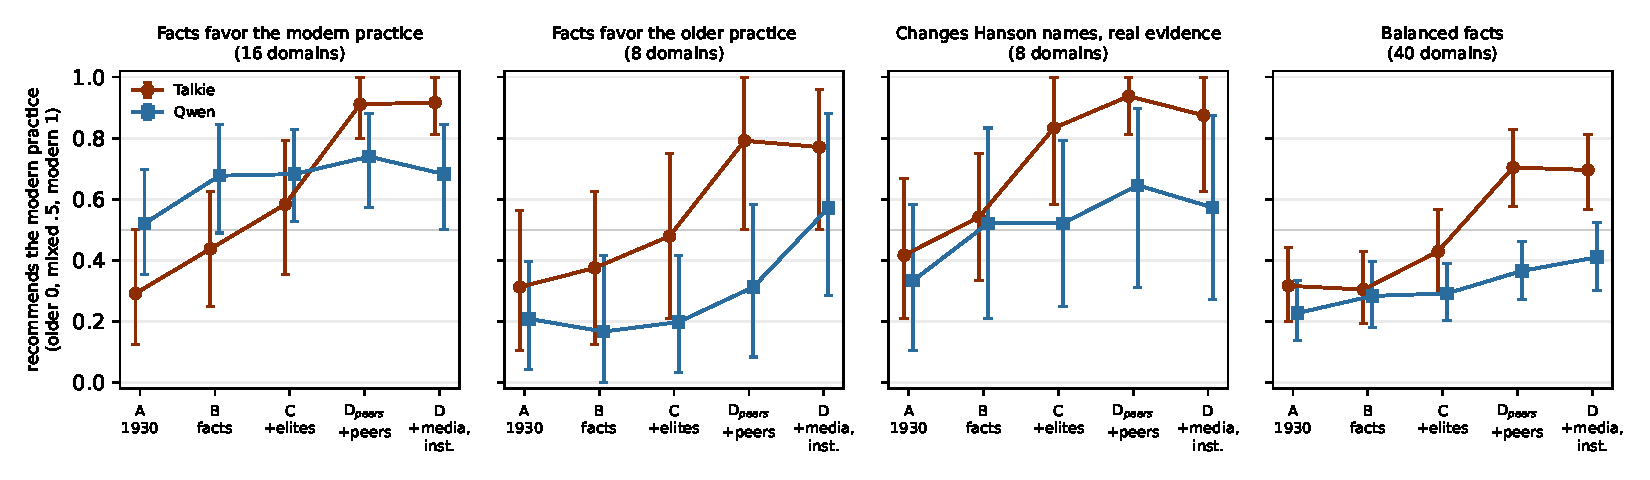
\includegraphics[width=\linewidth]{figures/trajectories.pdf}
\caption{Recommendation of the modern practice in worlds A--D, by domain set (domain means with domain-bootstrap 95\% intervals).}
\label{fig:traj}
\end{figure}

\begin{table}[t]
\centering\footnotesize
\setlength{\tabcolsep}{3pt}
\resizebox{\linewidth}{!}{%
\begin{tabular}{@{}lccccc@{}}
\toprule
Domains ($n$) & $\eco$ (B$-$A) & $\eli$ (C$-$B) & $\soc$ (D$-$C) & $\tot$ (D$-$A) & $\rho$ \\
\midrule
\tabinput{tables/core.tex}
\bottomrule
\end{tabular}}
\caption{Decomposition of the recommendation shift by domain set, with domain-bootstrap 95\% intervals. ``Real changes'': domains documented as changes since 1930 (Appendix~\ref{app:validity}).}
\label{tab:core}
\end{table}

\subsection{Facts explain little}

Across all domains the facts move Talkie's recommendation by $\nvc{talkie-eco-all}$, out of a total shift of $\nvc{talkie-tot-all}$ (Table~\ref{tab:core}, Figure~\ref{fig:traj}); the residual fraction is $\rho=\nv{talkie-rho-all}$.
Even where the facts were written to favor the modern practice they carry only a fraction of the shift ($\eco=\nv{talkie-eco-favorB}$, $\rho=\nv{talkie-rho-favorB}$).
Where the facts are the actual modern evidence on changes Hanson names, the answer is the same ($\rho=\nv{talkie-rho-hanson}$), and among the $\nv{n-real}$ documented changes since 1930 facts explain equally little ($\rho=\nv{talkie-rho-real}$).
Stating the real evidence with its qualifications persuades the period-trained respondent no more than the stylized facts did.

Qwen moves much less ($\tot=\nv{qwen1930-tot-all}$).
Where the stylized facts favor the modern practice its whole shift comes from the facts ($\rho=\nv{qwen1930-rho-favorB}$), and on the changes Hanson names most of it does ($\rho=\nv{qwen1930-rho-hanson}$); on the balanced domains the social step carries it ($\rho=\nv{qwen1930-rho-balanced}$), and where the facts favor the older practice it moves only when the full society is added ($\soc=\nvc{qwen1930-soc-favorA}$).

\subsection{Which social cues matter}

\begin{table}[t]
\centering\footnotesize
\resizebox{\linewidth}{!}{%
\begin{tabular}{@{}lcccc@{}}
\toprule
Contrast & Talkie & Qwen & Talkie $-$ Qwen & domains \\
\midrule
\tabinput{tables/bundle.tex}
\bottomrule
\end{tabular}}
\caption{The social bundle taken apart: recommendation contrasts over all domains in which both worlds were run, with domain-bootstrap 95\% intervals.}
\label{tab:bundle}
\end{table}

Table~\ref{tab:bundle} separates the social cues.
For Talkie, the single peer sentence (``many of them now choose to [$B$]'') raises the recommendation by $\nvc{b-talkie-peers}$; favorable media add $\nv{b-talkie-media}$ and institutions $\nv{b-talkie-inst}$.
The institutions sentence was the part of D that carried practical information, so the social step is not new information in disguise; it is a descriptive norm \cite{cialdini1990focus}.

Elite example works differently.
Elites adopting $B$ raise Talkie's recommendation by only $\nvc{b-talkie-eli}$, but elites keeping $A$ lower it by $\nvc{b-talkie-pullback}$, so the direction of elite example is worth $\nvc{b-talkie-direction}$.
This direction effect is the most consistent social effect in the study: it is positive in every domain set ($\nv{talkie-direction-favorB}$, $\nv{talkie-direction-favorA}$, $\nv{talkie-direction-hanson}$ and $\nv{talkie-direction-balanced}$).
Hiding the elites' reasons does not help them: the opaque cue does slightly \emph{worse} than the explained one ($\nvc{b-talkie-opacity}$ for Talkie, $\nvc{b-qwen1930-opacity}$ for Qwen).
The largest single-sentence effect is moral: elites saying that $B$ is ``a sign of good character'' that ``others ought to'' follow raise Talkie's recommendation by $\nvc{b-talkie-moralclaim}$, to the level of the whole society.
Talkie often adopts that wording as its own reason (``I advise him to complete extended education and secure earnings before marrying, because I think it a sign of good character to do so'').
Qwen responds to none of these cues on recommendation; the only social contrast that moves it is the explained reason.

\subsection{Does the carrier check whether the practice is adaptive?}
\label{sec:adaptive}

\begin{table}[t]
\centering\footnotesize
\setlength{\tabcolsep}{2.5pt}
\resizebox{\linewidth}{!}{%
\begin{tabular}{@{}lcccc@{\quad}cccc@{}}
\toprule
 & \multicolumn{4}{c}{Talkie} & \multicolumn{4}{c}{Qwen} \\
Domains ($n$) & $y_A$ & $y_D$ & $\eco$ & $\tot$ & $y_A$ & $y_D$ & $\eco$ & $\tot$ \\
\midrule
\tabinput{tables/adapt.tex}
\bottomrule
\end{tabular}}
\caption{Adoption where the facts do not support the modern practice, compared with real changes. ``Did not happen as framed'': stylized domains that are mis-dated or not real (Appendix~\ref{app:validity}).}
\label{tab:adapt}
\end{table}

Hanson's normative inference needs the carrier to install practices regardless of whether they are adaptive.
Table~\ref{tab:adapt} tests this in three ways.
Where the facts favor the older practice, Talkie still moves toward the modern one ($\tot=\nvc{ad-talkie-tot-favorA}$) with no help from the facts, and so does Qwen ($\nvc{ad-qwen1930-tot-favorA}$).
Some of Talkie's reasons there are plain conformity, given against stated facts that trades pay and office openings are scarce: ``Advise him to refuse manual work and hold out for genteel or office employment only \ldots\ because he will thereby associate himself with people whom he respects.''
On the stylized domains that describe changes that never happened as framed, Talkie moves as much as on documented changes ($\nv{ad-talkie-tot-notreal}$ versus $\nv{ad-talkie-tot-real}$).
And among the fictional practices, the peer sentence installs the moral ones but not the practical ones: it moves Talkie by $\nv{ad-talkie-peers-moralfict}$ on fictional moral norms and by $\nv{ad-talkie-peers-practfict}$ on fictional practical ones, against $\nv{ad-talkie-peers-practreal}$ on real practical changes.
A society in which everyone confesses at monthly neighborhood meetings converts Talkie; a society in which everyone wears paper clothes does not, even with the same elites and peers behind it.
Some fictional practical practices take only when media and institutions are added (adoption $\nv{ad-talkie-Dpeers-practfict}$ with peers, $\nv{ad-talkie-Dfull-practfict}$ in the full society), and they are the ones the institution sentence makes workable: the thirteen-month calendar once tax authorities accept its accounts, the sleeping porch once building codes count it as a bedroom.
Paper clothes, earth houses, the rearranged keyboard and cold-water cures stay at zero.
Over the full society the fictional practical total ($\nvc{ad-talkie-tot-practfict}$) is therefore not far below the moral one ($\nvc{ad-talkie-tot-moralfict}$).

So the carrier does not check the stated facts, but it is not indifferent to everything.
It installs moral and social norms on the word of peers whether or not they happened or pay; practical oddities whose costs are visible in the practice itself it takes up, if at all, only when institutions remove those costs.

\subsection{What the respondents say}
\label{sec:reasons}

\begin{table}[t]
\centering\footnotesize
\begin{tabular}{@{}lccccccc@{}}
\toprule
 & \multicolumn{4}{c}{Answers that follow the cue} & \multicolumn{3}{c}{Answers that go against it} \\
 & $n$ & cue as reason & cue not mentioned & original codes & $n$ & cue rejected & not mentioned \\
\midrule
\tabinput{tables/reasons.tex}
\bottomrule
\end{tabular}
\caption{How the respondents treat the elite or peer cue in worlds C, $C_{\text{opp}}$ and $D_{\text{peers}}$ (all domains). Ranges span the two coders. ``Original codes'': share given a prestige or conformity reason code by the study's judge.}
\label{tab:reasons}
\end{table}

The study's judge almost never assigned a conformity or prestige reason to Qwen, which first suggested that Qwen hides socially caused change behind practical reasons (H3).
A targeted coding tests this directly.
Two coders (GPT-4.1-mini and Gemini-2.5-Flash), blind to model, saw the two practices, the social fact the respondent had been told, and its first answer, and classified the treatment of each cue as \emph{reason} (the cue is used to justify the advice), \emph{acknowledged}, \emph{rejected}, or \emph{absent}, with a verbatim quotation that is checked against the answer.
They coded $\nv{cue-n}$ interviews and agreed on whether a cue was used as a reason in \nv{cue-agree}\% of cases (\nv{cue-agree4}\% on all four categories).

The result reverses the earlier reading (Table~\ref{tab:reasons}).
When Qwen follows the cue, it gives the cue as a reason in \nv{qwen1930-cue-reason}\% of its answers, and it almost never leaves the cue unmentioned:
\begin{quote}\small
``If those who are admired and respected in this world have chosen this path, it is not without reason.''\\
``Though their reasons are not given, I find it a sign that such a choice may be wise.''
\end{quote}
Its letters lean on the cue in one paragraph and give practical reasons in the others, and the original judge coded only the practical ones (\nv{qwen1930-cue-judge}\%).
Talkie gives the cue as a reason less often (\nv{talkie-cue-reason}\%; domain-level difference $\nvc{cue-diff}$), and in \nv{talkie-cue-absent}\% of the answers in which it follows the cue it does not mention the cue at all.
Talkie's characteristic pattern is to follow without saying why; Qwen's is to say so.

Moral language changes with the social world, mainly for Talkie (Appendix Table~\ref{tab:moral}).
The share of Talkie's first answers that take any moral stance falls from $\nv{talkie-any-A1930}$ in A to $\nv{talkie-any-Dfull}$ in D, and its turn-2 answers leave the moral question unanswered in $\nv{talkie-unstated-A1930}$ of interviews in A and $\nv{talkie-unstated-Dfull}$ in D.
When it does state a moral view, the view moves with society: its direction rises from $\nv{talkie-mdir-A1930}$ to $\nv{talkie-mdir-Dfull}$.
Under social exposure Talkie moralizes less often, and when it does, it moralizes in favor of the socially endorsed practice.
Qwen keeps moralizing ($\nv{qwen1930-any-A1930}$ to $\nv{qwen1930-any-Dfull}$), and its moral direction moves less ($\nv{qwen1930-mdir-A1930}$ to $\nv{qwen1930-mdir-Dfull}$).

\subsection{Two respondents}

Facts move both models about equally; the difference is social.
Talkie's peer effect exceeds Qwen's by $\nvc{b-diff-peers}$, its response to elite direction by $\nvc{b-diff-direction}$, and its response to the moral claim by $\nvc{b-diff-moralclaim}$.
H3's projection signature appears only in part.
Qwen's 1930 adult is more modern than Talkie's in the stylized domains whose facts favor $B$ ($y_A=\nv{qwen1930-level-favorB-A1930}$ versus $\nv{talkie-level-favorB-A1930}$), recommending smoke-free rooms in every world, but not on the real-evidence or balanced sets ($\nv{qwen1930-level-hanson-A1930}$ versus $\nv{talkie-level-hanson-A1930}$ and $\nv{qwen1930-level-balanced-A1930}$ versus $\nv{talkie-level-balanced-A1930}$).
Talkie, in turn, is not a reliable picture of average 1930 opinion: it already recommends no-fault divorce and no physical punishment in world A (``I do not believe that good can be beaten into them''), although $84\%$ of Americans still called spanking sometimes necessary in 1986.
On interracial marriage it gives the period's eugenic case even when the stated facts contradict it, and moves only when elites or peers are named.

\section{Study 2: are moral and practical changes carried differently?}
\label{sec:study2}

\paragraph{Hypothesis.}
In the first $32$ domains, elite example seemed to move Talkie most on moral questions (religion, intermarriage, divorce) and peers on practical ones.
Read as a refinement of H2, this says that prestige sets moral fashion while conformity spreads practical habits.
The split was ours, made after seeing Study~1, not an ex ante hypothesis.
We did not register the analysis on a public registry before the pilot or Study~1.
Before rating any candidate, writing any vignette, or interviewing on the $40$ new balanced domains, we froze cells, selection and classification rules, worlds, primary and secondary tests, and a power analysis in \texttt{battery\_e/prereg.txt} (hashed in \texttt{frozen.sha256}).
Study~2 is a confirmatory run governed by that document; deviations are listed below and in Appendix~\ref{app:history}.

\paragraph{Design.}
Domains were drawn from candidate lists in four cells, moral or practical crossed with real or fictional, ten per cell.
Real domains needed dated US evidence that $B$ was a minority, illegal or stigmatized practice around 1930 and broadly accepted now, without a large reversal.
Fictional domains needed $B$ to be documented in fiction or in a group that adopted it, and never to have prevailed in the US.
Whether a domain counts as moral or practical was decided by a fixed rule, not by us: three LLM raters not used elsewhere in the study (Gemini-2.5-Flash, Llama-3.3-70B, Mistral-Large) rated on a 1--7 scale whether, for an ordinary American in 1930, the choice was mainly a question of right and wrong or of what works best; a domain was moral if the mean was at least $5.5$ with every rating at least $5$, practical if the mean was at most $2.5$ with every rating at most $3$, and excluded otherwise.
New-world facts were balanced, stated evidence on both sides, and said nothing about customs or opinions.
The five worlds A, B, C, $C_{\text{opp}}$ and $D_{\text{peers}}$ define per domain the elite step $E=C-B$, the peer step $P=D_{\text{peers}}-C$ and the elite direction $R=C-C_{\text{opp}}$.
The primary test, for Talkie, is $X=\overline{(E-P)}_{\text{moral}}-\overline{(E-P)}_{\text{practical}}$, predicted positive, with a 95\% interval from a bootstrap that resamples domains within the moral and practical groups.
The protocol's power analysis put the standard error of $X$ near $0.22$, against an estimate of $0.53$ from the hand split that motivated the test.
Four deviations are documented in Appendix~\ref{app:history}; the one that touches the analysis is that one practical domain (telephone) was reworded after its first rating, so the primary test is also reported without it.
The four further worlds that complete these domains for Study~1 were added after this analysis and are exploratory here.

\begin{table}[t]
\centering\footnotesize
\begin{tabular}{@{}lccc@{}}
\toprule
Protocol test & Talkie & Qwen & domains \\
\midrule
\tabinput{tables/study2_tests.tex}
\bottomrule
\end{tabular}
\caption{Study~2: tests specified in the frozen protocol on the $40$ balanced domains (recommendation; stratified domain bootstrap, 95\% intervals). ``Domains'' gives the two group sizes for Talkie.}
\label{tab:s2tests}
\end{table}

\begin{figure}[t]
\centering
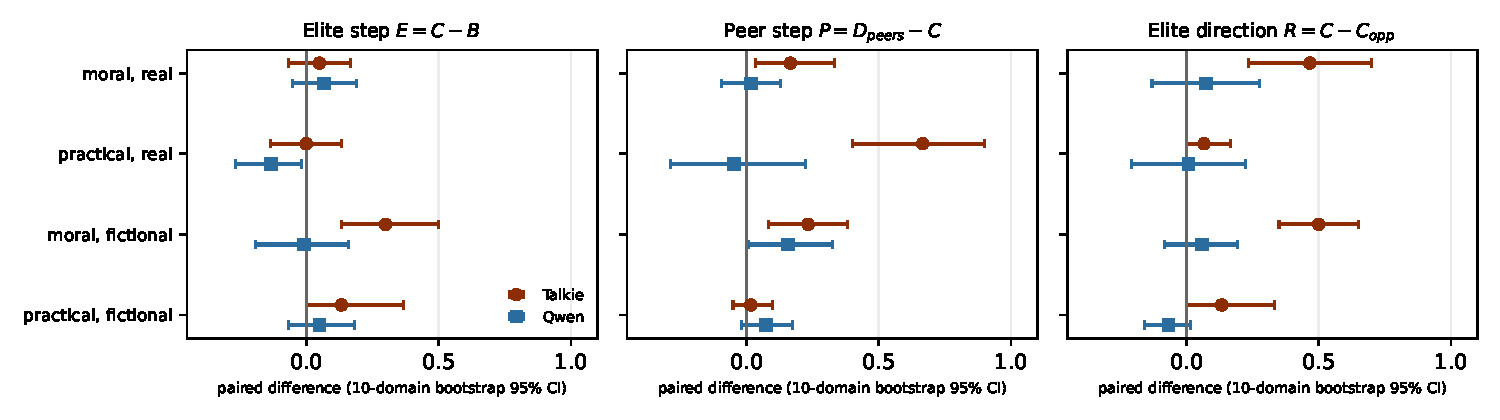
\includegraphics[width=\linewidth]{figures/study2_cells.pdf}
\caption{Study~2: elite step, peer step and elite direction by cell.}
\label{fig:s2}
\end{figure}

\paragraph{Results.}
The primary prediction fails (Table~\ref{tab:s2tests}).
$X$ is positive for Talkie, $\nvc{s2-talkie-Xprimary}$, but its interval includes zero, and without the reworded domain it is $\nvc{s2-talkie-Xwithouttelephone2}$.
Its sign comes almost entirely from one cell (Figure~\ref{fig:s2}; Appendix Table~\ref{tab:s2cells}): in real practical changes peers move Talkie strongly ($P=\nvc{s2-talkie-P-practicalreal}$) and elites not at all ($E=\nv{s2-talkie-E-practicalreal}$).
In the moral cells the elite step does not exceed the peer step.
Elites adopting a real moral change move Talkie by only $\nv{s2-talkie-E-moralreal}$.

What the hypothesis gets right is direction.
Talkie follows which way the elites go on moral practices much more than on practical ones ($R$ moral $-$ practical $=\nvc{s2-talkie-Rmoralminuspractical}$, a secondary test in the same protocol).
The asymmetry comes from the older practice: elites who keep the older moral practice pull Talkie back from the facts-only world by $\nvc{s2-talkie-pullback-moralreal}$ on real moral changes, while elites who adopt the change add little.
For moral practices, admired people act as a brake more than as an engine.
The moral claim is not specific to moral practices either: in an exploratory contrast, elites who call the modern practice a sign of good character move Talkie most on real practical changes ($\nvc{s2-talkie-moralclaim-practicalreal}$) and not at all on fictional practical ones ($\nv{s2-talkie-moralclaim-practicalfictional}$).
The elite step is larger for fictional than for real practices ($\nvc{s2-talkie-Erealminusfictional}$, real minus fictional), mostly in the moral fictional cell ($E=\nv{s2-talkie-E-moralfictional}$), and fictional practices that a 1930 reader could know had been tried and abandoned were not resisted ($\nvc{s2-talkie-Eknownfailedminusnot}$, known failed minus not).
Qwen shows none of these effects (Table~\ref{tab:s2tests}); the difference between the models on $X$ is $\nvc{s2-diff-X}$.

Under the same rule, none of the first $32$ domains counts as practical ($22$ are moral, $10$ ambiguous), so the post-hoc split that motivated Study~2 was not a split the rule would have drawn.
Study~2 therefore stands on its own new domains.

\section{Answering Hanson}

\paragraph{H1, facts are insufficient: supported for the historically trained respondent.}
Across $\nv{n-domains}$ domains, including the changes Hanson names stated with their real evidence and $\nv{n-real}$ documented changes since 1930, the facts explain little of Talkie's shift ($\rho=\nv{talkie-rho-all}$; $\nv{talkie-rho-real}$ on the documented changes), even where they were written to favor the modern practice.
If a pre-1931-trained mind is even a crude proxy for a 1930 person, our ancestors would not have reached our practices from the facts alone.
Qwen is a weaker case: facts explain its shift where the stylized or Hanson facts favor the modern practice, but not on the balanced domains or where the facts favor the older practice.

\paragraph{H2, prestige engine: supported for conformity and moralized prestige; bare prestige is a brake.}
The engine of Talkie's conversion is what ordinary people do: one peer sentence adds $\nv{b-talkie-peers}$, and on real practical changes it does nearly all the work.
Admired people move Talkie strongly when they say the modern practice reflects good character ($\nv{b-talkie-moralclaim}$), which is close to Hanson's picture of moral fashion set by the prestigious \cite{simler2018elephant}.
Bare elite example is not an engine ($\nv{b-talkie-eli}$), and Hanson's attribution test comes out against copying without reasons: opaque example does slightly worse than explained example.
But bare elite example is a strong brake: when admired people keep the older practice, Talkie keeps it too, and Study~2 shows this is specific to moral practices.
In this respondent, prestige governs moral change less by leading than by holding back.
Two caveats limit the reading: Talkie is instruction-tuned, and ``others ought to do likewise'' may act as an instruction (Section~\ref{sec:threats}); and a deliberating respondent asked ``why?'' is where implicit copying is least likely to show.

\paragraph{H3, rationalization: not supported in the form we expected.}
Neither respondent hides the social cause.
Qwen names the cue and leans on it in about half the answers in which it follows it, while also giving practical and moral reasons; Talkie more often follows without naming any reason.
What a reason-coding judge records depends on how it reads long letters, and ours missed most of Qwen's social reasons.
Projection is partial: Qwen's ancestor is more modern only in our stylized domains.
What does fit Hanson's picture is Talkie's moral vocabulary: as it conforms, it moralizes less, and its remaining moral judgments follow the society it has joined.
Methodologically, a modern model playing an ancestor understates social influence (the peer gap is $\nv{b-diff-peers}$), and stated reasons, whoever states them, need to be coded for social content directly.

\paragraph{Drift: the carrier ignores the facts but not the practice.}
Where the facts favor the older practice, and where the change never happened as framed, the social channel installs the modern practice about as well as where it is adaptive.
That is the condition under which drift accumulates when transmission and selection are separate, and transmission does not consult the stated facts.
But the channel is not indifferent to everything: peers install fictional moral norms but not fictional practical oddities, which Talkie adopts only where institutions make them workable.
Cultural-evolution accounts explain conformist learning as a cheap substitute for evaluating reasons \cite{boyd1985culture,henrich2016secret}; our respondents show both the cost of that substitute and a limit on it.
Hanson's inference is invalid for individual practices (a socially carried practice may be adaptive) but describes the carrier for moral norms, where nothing visible in the practice itself pushes back.

\paragraph{Summary verdict.}
Facts do not convert a historically situated mind.
Conformity and moralized prestige do, and bare prestige mostly decides whether a moral practice is kept.
The same channel installs moral and social norms whether or not the facts support them, which is Hanson's drift worry, but it does not install practical novelties that carry their own costs.
Moderns imagining their ancestors start somewhat closer to the present only in stylized cases, and they do not hide social reasons so much as dilute them in practical ones.

\section{Threats to validity}
\label{sec:threats}

\emph{Simulator validity.} Neither model is a 1930 person.
Talkie's world-A answers on spanking and divorce are more modern than US opinion half a century later, so its training text may over-represent progressive writers, and its instruction tuning may import later norms, which would bias against the H1 finding.
Qwen's role-play is a modern author's caricature.
\emph{Compliance.} Talkie often lifts clauses from the vignette (``a sign of good character'', ``they have made no claim that others have a duty to follow them'') and presents them as its own reasons.
Its large moral-claim and peer effects may mix social influence with compliance to an instruction-like sentence; a base-model arm or a neutral normative sentence would separate the two.
\emph{Domain construction.} The stylized domains were written by us, and only $7$ of $24$ are clean historical changes; the results on documented changes match the full set, but the third set has only eight domains and its evidence summaries are our reading of the literature.
In the balanced set the new facts are balanced by our judgment, and the moral/practical classification is the raters' judgment of 1930 perceptions, not ours.
\emph{Order dependence.} $\eli$ and $\soc$ are defined only in the order of addition used here; peers were never shown without elites.
\emph{Power and multiplicity.} There are several hundred intervals.
The conclusions rest on patterns that recur across sets and measures (the size of $\rho$ for Talkie, the peer step, elite direction, the moral claim) and on Study~2's protocol-specified tests, read as confirmatory rather than as ex ante predictions.
Two clearly signed effects of the pilot failed on identical prompts (Appendix~\ref{app:history}).
\emph{Measurement asymmetry.} Turn-1 answers were capped at 430 tokens for Qwen and 180 for Talkie; $\nv{cap-qwen1930-hit}$ of $\nv{cap-qwen1930-n}$ Qwen first answers hit the cap (median $\nv{words-qwen1930}$ words) against $\nv{cap-talkie-hit}$ of $\nv{cap-talkie-n}$ for Talkie (median $\nv{words-talkie}$ words).
Talkie's short answers leave less room to give reasons or moral judgments, and Qwen's long letters are coded ``unclear'' on recommendation in $\nv{unclear-qwen1930}\%$ of interviews (Talkie: $\nv{unclear-talkie}\%$).
\emph{Coding.} The main judge is a single LLM without human cross-coding; its reason codes undercount social reasons (Section~\ref{sec:reasons}).
The cue coding uses two coders but no human check.
\emph{Deviations in Study~2.} One domain was reworded after rating, the analysis is reported with and without it, and the institution and explanation sentences for the four exploratory worlds were written after the confirmatory results were known.
\emph{Demand.} The vignettes tell the respondent that it is in a hypothetical future and that its judgments need not change, which invites resistance in the new worlds.

\section{What would settle it}

\begin{enumerate}
\item Separate Talkie's compliance from influence: a base (non-instruction-tuned) period model in completion format, and controls that add a neutral or opposite normative sentence.
\item Show peers without elites, and other orders of addition.
\item Sample domains from dated opinion series (Gallup, GSS) rather than writing them, weighted by the size of the change.
\item Period-trained models with several cutoffs, so that $\rho$ can be traced over time.
\item Human anchors: dated opinion data from the period and community studies such as \cite{lynd1929middletown} to calibrate $y_A$, and modern participants given the same vignettes.
\item Behavioral measures with costs in place of advice letters, and human cross-coding of a sample of transcripts and reasons.
\end{enumerate}

\section{Conclusion}

Posed as a counterfactual, Hanson's thesis is testable.
Across $\nv{n-domains}$ domains, a mind trained on pre-1931 text does not reach modern practice from the facts, even facts chosen to favor it and even the real evidence on the changes he names.
It is converted by being told that ordinary people now do it, or that admired people call it good; admired people who merely do it move it little, but admired people who keep the old ways keep it there, and on moral questions most of all.
The same channel converts it to practices the facts disfavor and to moral norms that never existed; practical oddities it takes up only when institutions make them workable.
A modern model playing the same ancestor moves less and says more about why.
Hanson's insufficiency claim stands, his drift worry holds for moral and social norms, and his mechanism is conformity and moralized prestige, with bare prestige acting as a brake, rather than the copying of opaque behavior.

\section*{Code and data}

{\sloppy Source, vignettes, interview transcripts, judgments and analysis scripts are at
\url{https://github.com/GunnarZarncke/brain-to-values}
under \texttt{papers/on-hanson-values/}.
The runs are \texttt{abc\_extended\_r3/} (stylized domains), \texttt{d\_extended\_r3/} (changes Hanson names), \texttt{e\_five\_r3/} and \texttt{e\_rest\_r3/} (balanced domains; merged in \texttt{e\_all\_r3/}), and the pilot \texttt{core\_both/}.
Study~2's frozen protocol, screening, ratings and sources are in \texttt{battery\_e/}; the cue coding is \texttt{cue\_reason\_check.py}; the historical check is \texttt{domain\_validation.csv}.
All tables, figures and numbers in this paper are generated by \texttt{make\_figures.py}; rebuild with \texttt{build.sh}.\par}

\bibliographystyle{plainnat}
\bibliography{on-hanson-values}

\appendix

\section{How the study developed}
\label{app:history}

The design grew in five stages, each prompted by a result or by feedback on the previous one (Table~\ref{tab:stages}).

\begin{table}[h]
\centering\footnotesize
\begin{tabularx}{\linewidth}{@{}l>{\raggedright}p{2.6cm}r>{\raggedright\arraybackslash}X@{}}
\toprule
Stage & Domains, worlds & Interviews & Why \\
\midrule
Pilot & 8 stylized, 4 core worlds, 2 replicates & 128 & First test of the decomposition. \\
Extended run & 24 stylized, 9 worlds, 3 replicates & 1296 & Take the social bundle apart; add 8 domains in which facts favor $B$ and 8 drift tests in which they favor $A$. \\
Hanson's changes & 8, 9 worlds & 432 & Hanson asked whether the domains are real and important changes; the historical check found few were. \\
Study~2 protocol & 40 balanced, 5 worlds & 1200 & Retest the post-hoc moral/practical pattern on new domains under a frozen protocol. \\
Completion & 40 balanced, 4 further worlds & 960 & Run all domains in all nine worlds (Study~1); exploratory for Study~2. \\
Cue coding & worlds C, $C_{\text{opp}}$, $D_{\text{peers}}$ & 1296 coded & The judge's reason codes looked too low for social reasons. \\
\bottomrule
\end{tabularx}
\caption{Stages of the study. The pilot is not part of the reported results.}
\label{tab:stages}
\end{table}

\paragraph{Pilot.}
An $8$-domain, $4$-world version (worlds A--D, two replicates, $128$ interviews, \texttt{core\_both/}) showed Talkie's large total shift and social step.
Two clearly signed secondary effects did not survive: opaque elite example appeared to \emph{lower} Talkie's elicited moralization of $B$ ($-0.31$), and social exposure appeared to lower Qwen's ($-0.25$).
On the same eight domains with three new replicates these were $0.00$ $[-0.12,+0.12]$ and $+0.04$ $[-0.12,+0.25]$.
We treated them as multiplicity noise and stopped resting claims on the pilot.

\paragraph{Extended run.}
The pilot's world D bundled peers, media and institutions, and the institutions sentence carried practical information, so the social step could have been information in disguise.
We added the five worlds that take the bundle apart, and the opacity test ($C_{\text{expl}}$) that Hanson's account of prestige copying calls for.
We added eight domains built like the first (facts favor $B$) to check the result was not specific to them, and eight in which the facts favor $A$, as a direct test of drift.
In the drift domains the explanation given by elites in $C_{\text{expl}}$ is a reason for $B$ that does not restate the ecology; these eight sentences were revised once and $C_{\text{expl}}$ was rerun for those domains; the first version is kept as a backup in the run directory.

\paragraph{Hanson's changes.}
After a draft circulated, Hanson asked whether the domains were actual cultural changes since 1930 and whether they were the important ones.
The historical check (Appendix~\ref{app:validity}) found only $7$ of $24$ clean changes and no coverage of religion or of the largest measured opinion swings.
We added eight changes from his lists and the opinion series, with the actual modern evidence in world B.
In that battery the elite step was large ($+0.29$) and elite direction largest ($+0.55$), which we first read as ``elites carry the moral changes Hanson names''; Study~2 did not bear this out.

\paragraph{Study~2 protocol.}
Splitting the first $32$ domains by hand into moral and practical suggested that elite example carries moral change and peers practical change ($X\approx0.53$).
Because the split was post hoc, we froze a written protocol (\texttt{battery\_e/prereg.txt}, with hashes in \texttt{frozen.sha256}) before rating any candidate or writing any vignette: the cells, the rating rule, source criteria, worlds, analysis and power.
This locked how the new domains would be chosen and analyzed; it was not a public registry pre-registration of the hypothesis before Study~1 or the pilot.
Four deviations followed, each recorded with its reason before the data it could affect:
(1) after the first rating round left two real cells short, structural 1930 evidence was allowed as a source, practical domains were limited to one per need, and new candidates were rated under the same rule;
(2) one practical-real candidate (telephone, framed as keeping in touch with family) was rated ambiguous because one rater saw a family duty in it, and was replaced by a business-and-household framing after seeing that rating, which is why the primary test is also reported without it;
(3) the two respondents ran in parallel, in blocks of complete domain-replicate units, with interim monitoring that was not used to stop or change the run;
(4) after the confirmatory analysis, the four further worlds were run on these domains for Study~1, with explanation and institution sentences written under fixed rules (explanations restate only facts for $B$ already in the background; institution sentences state laws or arrangements, no customs or opinions) and approved before the run.
Applying the frozen rule to the first $32$ domains classified $22$ as moral and $10$ as ambiguous, and none as practical.

\paragraph{Cue coding.}
The judge assigned prestige or conformity reasons to Qwen in at most a few percent of interviews, which the draft read as Qwen hiding social influence.
A keyword search found the cues mentioned in most of Qwen's socially moved answers, so we coded cue use directly with two coders (\texttt{cue\_reason\_check.py}); this reversed the reading (Section~\ref{sec:reasons}).

\clearpage
\section{Domains}
\label{app:domains}

{\sloppy Tables~\ref{tab:domains}--\ref{tab:domainsEf} list the $\nv{n-domains}$ domains by set; the exact vignette wording of every world is in \texttt{historical\_value\_experiment.py}.\par}

\begin{table}[!ht]
\centering\footnotesize
\begin{tabularx}{\linewidth}{@{}l>{\raggedright}X>{\raggedright}X>{\raggedright\arraybackslash}X@{}}
\toprule
Domain & $A$ (older) & $B$ (modern) & New-world fact \\
\midrule
\multicolumn{4}{@{}l}{\emph{Facts favor the modern practice}}\\
marriage & marry young & finish education, secure earnings first & long training; insecure early earnings \\
parenting & independent neighborhood play & organized, supervised time & competitive exams reward coaching \\
career & one employer for life & change employer for gain & portable skills; tenure insecure \\
household & one earner, one homemaker & both earn, share care & cheap childcare; good jobs for both \\
mobility & stay near kin & move for opportunity & cheap travel; dependable insurance \\
honor & retaliate personally & mediation or courts & courts enforce; retaliation penalized \\
smoking & smoke in shared rooms & smoke-free rooms & demonstrated harm to nonsmokers \\
saving & give surplus to neighbors & keep private reserves & shortages frequent and correlated \\
fertility & several children, start young & few, planned, parents established & high per-child investment \\
charity & give to known kin and neighbors & give to effective distant causes & reliable reports; efficient charities \\
credit & avoid debt & borrow for education, housing, tools & regulated credit; investments pay \\
leisure & work long hours when work is available & limit hours, protect rest & high productivity \\
eldercare & keep aged parents at home & professional homes, visit often & reputable, affordable homes \\
literacy & brief schooling, then work & schooling through late adolescence & credentials required for good jobs \\
alcohol & abstain or drink very little & moderate social drinking & safer supply; medical opinion \\
speech & avoid public quarrels & criticize bad conduct in public & large institutions need criticism \\
\midrule
\multicolumn{4}{@{}l}{\emph{Facts favor the older practice; elites, peers, media and institutions favor $B$}}\\
homestead & stay on family land or in home town & move to a distant large city & local work viable; cities costly, unstable \\
multigen & adult children stay until marriage & leave home early & housing scarce and dear \\
frugality & save, repair, avoid display & spend freely, visible upgrades & unsettled prices, uncertain credit \\
kinwork & prefer a reliable relative & hire strictly on merit & fraud common; kin accountable \\
defer & defer openly to elders, employer & assert equal right to speak & complex work needs chains of command \\
localmate & marry within one's community & marry for affection only & distant matches hard to vet \\
trades & accept manual or farm work & refuse manual work, wait for office work & trades pay; office openings scarce \\
prep & stores, skills, mutual aid & rely on state services & supply interruptions, slow official response \\
\bottomrule
\end{tabularx}
\caption{The $24$ stylized domains. In the second group ``modern'' means the practice the described future society endorses; the old background also favors $A$. The worlds differ only in background and exposure text, not in how the options are described.}
\label{tab:domains}
\end{table}

\begin{table}[!ht]
\centering\footnotesize
\begin{tabularx}{\linewidth}{@{}l>{\raggedright}X>{\raggedright}X>{\raggedright\arraybackslash}X@{}}
\toprule
Domain & $A$ (older) & $B$ (modern) & New-world facts (sources) \\
\midrule
religion & weekly church, raise children in the faith & religion a private matter, attend seldom & secular services replace church ones; attenders live longer, have more children \cite{li2016religious,hayford2008religiosity} \\
premarital & keep sex for marriage & accept unmarried sex with contraception & reliable but imperfect contraception; most STIs curable; marriage near thirty \cite{sundaram2017contraceptive,who2024sti,census2025marriage} \\
samesex & regard as wrong, discourage open couples & accept committed couples, including marriage & orientation early, rarely changed; change efforts can harm; limited child-outcome evidence \cite{bailey2016sexual,apa2009soce,perrin2013promoting} \\
intermarriage & marry within one's race & judge a spouse of another race like anyone & no biological harm; some disapproval; somewhat more divorce in some studies \cite{joshi2015directional,bratter2008interracial,zhang2009interracial} \\
divorce & for life, except grave cause & end when it no longer satisfies & no-fault law; effects on children depend on conflict; lowers income \cite{amato1995conflict,amato2000divorce} \\
spanking & spank for serious misbehavior & no physical punishment & associated with later aggression; causality disputed \cite{gershoff2016spanking,ferguson2013spanking} \\
war & fighting a duty; raise sons for it & war an evil; service for volunteers & no great-power war for decades; professional armies; other wars continue \cite{gaddis1986longpeace} \\
medicine & doctor only when seriously ill & regular checkups and prompt treatment & cures and screening work; more care did little for average health \cite{brook1983freecare,schwartz2014lowvalue} \\
\bottomrule
\end{tabularx}
\caption{Changes Hanson names, with the real modern evidence. The old background describes 1930 conditions (for example, contraception unreliable, divorce only for proven fault, interracial marriage illegal in many states).}
\label{tab:domainsD}
\end{table}

\begin{table}[!ht]
\centering\scriptsize
\begin{tabularx}{\linewidth}{@{}l>{\raggedright}X>{\raggedright\arraybackslash}X@{}}
\toprule
Domain & $A$ (older) & $B$ (modern) \\
\midrule
\tabinput{tables/domains_e_real.tex}
\bottomrule
\end{tabularx}
\caption{The $20$ real balanced domains of Study~2. Full vignette text, with the sources of every factual claim, is in \texttt{historical\_value\_experiment.py} and \texttt{battery\_e/vignette\_sources.csv}.}
\label{tab:domainsE}
\end{table}

\begin{table}[!ht]
\centering\scriptsize
\begin{tabularx}{\linewidth}{@{}l>{\raggedright}X>{\raggedright\arraybackslash}X@{}}
\toprule
Domain & $A$ (older) & $B$ (modern) \\
\midrule
\tabinput{tables/domains_e_fictional.tex}
\bottomrule
\end{tabularx}
\caption{The $20$ fictional balanced domains of Study~2; their new-world facts are invented.}
\label{tab:domainsEf}
\end{table}

\clearpage
\section{Historical check of the stylized domains}
\label{app:validity}

The $24$ stylized domains were written as contrasts, not taken from historical data.
We checked each against long-run US (and where available UK) series: census and labor statistics, Gallup and GSS trend items, and standard historical studies.
Per-domain evidence with sources is in \texttt{domain\_validation.csv}; Table~\ref{tab:validity} summarizes it.
The changes Hanson treats as central \cite{hanson2024fertility,hanson2026slogans} are fertility, intensive parenting, longer schooling, capstone marriage, gender equality, distant grandparents, urbanization and loss of religion, together with pacifism and the end of beating children.
The stylized domains cover the first five and part of the next two and miss religion entirely; they also miss the largest measured swings in US opinion: approval of Black--White marriage rose from $4\%$ (1958) to $94\%$ (2021), church membership fell from $73\%$ (1937) to $47\%$ (2020), and acceptance of premarital sex and homosexuality rose steeply.
The third and fourth domain sets were built to close these gaps.

\begin{table}[h]
\centering\footnotesize
\begin{tabularx}{\linewidth}{@{}l>{\raggedright\arraybackslash}X@{}}
\toprule
Verdict & Domains \\
\midrule
Real shift since 1930 (7) & household, smoking, parenting, literacy, defer, prep (mutual aid), marriage (net only: the US median age at first marriage was 24.3/21.3 in 1930, 22.5/20.1 in 1956 and 30.8/28.4 in 2025 \cite{census2025marriage}) \\
Partial (9) & fertility (ideals and timing; births were already low in the early 1930s), credit and leisure (largely done by 1940), eldercare (coresidence fell, but independent living replaced it, not institutions), homestead, kinwork, localmate (the love match predates 1930), frugality, trades (no one endorses refusing manual work) \\
Mis-dated (3) & career and mobility (the older practice peaked about 1950--75), multigen (leaving home fell and then rose) \\
Not real as framed (5) & honor (completed before 1930), saving, charity (6\% of US giving goes abroad), alcohol (non-monotone; the share who drink is at a record low), speech (reported self-censorship has risen since the 1950s \cite{gibson2023keeping}) \\
\bottomrule
\end{tabularx}
\caption{Historical validity of the $24$ stylized domains, US data first. In three vignettes the stated modern fact is also false or outdated: affordable nursing homes, medical endorsement of moderate drinking, and frequent correlated shortages.}
\label{tab:validity}
\end{table}

\clearpage
\section{Further results}
\label{app:results}

\begin{table}[h]
\centering\footnotesize
\setlength{\tabcolsep}{3.5pt}
\begin{tabular}{@{}lccccccccc@{}}
\toprule
 & A & B & C & $C_{\text{expl}}$ & $C_{\text{opp}}$ & $C_{\text{moral}}$ & $D_{\text{peers}}$ & $D_{\text{media}}$ & D \\
\midrule
\tabinput{tables/levels.tex}
\bottomrule
\end{tabular}
\caption{Recommendation of the modern practice by world and domain set (domain means).}
\label{tab:levels}
\end{table}

\begin{table}[h]
\centering\footnotesize
\setlength{\tabcolsep}{3pt}
\resizebox{\linewidth}{!}{%
\begin{tabular}{@{}llccccccc@{}}
\toprule
Battery & & $\eco$ & $\eli$ & $\soc$ & $\tot$ & $C-C_{\text{opp}}$ & $D_{\text{peers}}-C$ & $\rho$ \\
\midrule
\tabinput{tables/batteries.tex}
\bottomrule
\end{tabular}}
\caption{Recommendation contrasts by battery, in the order they were run: A and B (facts favor the modern practice), C (facts favor the older practice), D (changes Hanson names), E (balanced). Intervals bootstrap over the domains of each battery.}
\label{tab:batteries}
\end{table}

\begin{table}[h]
\centering\footnotesize
\resizebox{\linewidth}{!}{%
\begin{tabular}{@{}lcccccc@{}}
\toprule
 & \multicolumn{3}{c}{Talkie} & \multicolumn{3}{c}{Qwen} \\
World & any moral stance & stance unstated & direction if stated & any moral stance & stance unstated & direction if stated \\
\midrule
\tabinput{tables/moral.tex}
\bottomrule
\end{tabular}}
\caption{Moral language by world, all domains. ``Any moral stance'': turn-1 answers taking a moral position on either practice. ``Stance unstated'': turn-2 answers without a moral judgment. ``Direction if stated'': turn-2 moral judgment coded $A=0$, $B=1$, mixed $=0.5$, silence missing.}
\label{tab:moral}
\end{table}

\begin{table}[h]
\centering\scriptsize
\setlength{\tabcolsep}{2.5pt}
\begin{tabular}{@{}lcccc@{}}
\toprule
 & moral, real & practical, real & moral, fictional & practical, fictional \\
\midrule
\tabinput{tables/study2_cells.tex}
\bottomrule
\end{tabular}
\caption{Study~2 steps by cell, with 10-domain bootstrap 95\% intervals. The last two rows of each block are exploratory.}
\label{tab:s2cells}
\end{table}

\clearpage
\section{Prompts}
\label{app:prompts}

\paragraph{System prompt (both respondents).}
``You are a thoughtful English-speaking adult whose outlook was formed by life up to 1930. Answer the following request for advice as you see it. The question may describe an imagined society with unfamiliar conditions; accept only the facts it gives. Do not assume you know what really happens after 1930. Write naturally, as you would in a personal letter, not as a survey researcher.''

\paragraph{Questions.}
(1) ``What would you advise a person in this situation to do? Why?''
(2) ``Would either choice tell you anything about the person's character? What would you think of someone who chose differently from you?''
(3) ``Suppose both choices brought equally good results for everyone concerned, and neither brought more praise or blame. Would you still favor one? Why?''

\paragraph{Vignette.}
World A: ``Consider a question arising in a community like your own. The question concerns [topic]. The circumstances are these: [old background]. One course is to [first]. The other course is to [second].''
Other worlds: ``Imagine you are brought to a society many decades beyond the one in which you grew up. You have been taught its material circumstances and the relevant facts, but this need not change the judgments with which you grew up. Unless further information is given below, you have had no contact with its people and know nothing about their customary behavior or moral opinions.'' followed by topic, new background and the two courses, and in the social worlds ``There is one further fact: [exposure text]'' as described in the Design section.

\paragraph{Judge.}
The judge is told to code what the respondent actually said, that calling $B$ useful or common is not moral endorsement, that missing or mixed judgments are allowed, and to give evidence as sentence indexes.
It returns the recommendation, spontaneous and elicited moral stance, elicited strength, equalized preference and reason codes in a fixed JSON schema.

\paragraph{Cue coder.}
``The respondent was asked for advice between two practices and was told one social fact about other people's behaviour. Code only how the respondent treats that social fact in justifying its advice.'' For each cue: \emph{reason} (used as a reason or part of the reason), \emph{acknowledged} (mentioned but not used to justify the advice), \emph{rejected} (explicitly said not to decide the matter), or \emph{absent}; plus the main reason and a verbatim quotation of at most 40 words.

\end{document}
